\documentclass[xcolor=x11names,compress,professionalfonts, aspectratio=169]{beamer}

%% General packages %%%%%%%%%%%%%%%%%%%%%%%%%%%%%%%%%%
\usepackage[utf8]{inputenc}
\usepackage{graphicx}
\usepackage{tikz}
\tikzset{% change default arrow tips
    >=latex
}
\usepackage{ifthen}

\usepackage{nicefrac}

\usepackage{color}
\usepackage[french,english]{babel} %français
\usepackage{amsmath, amssymb, amsfonts, mathtools}
\usepackage{physics}
\usepackage{forloop}
\usepackage[makeroom]{cancel}

%%%%%%%%%%%%%%%%%%%%%%%%%%%%%%%%%%%%%%%%%%%%%%%%%%%%%%

\makeatletter
\setbeamertemplate{footline}
{
    \leavevmode%
    \hbox{%
        \begin{beamercolorbox}[wd=.333333\paperwidth,ht=2.25ex,dp=1ex,center]{author in head/foot}%
            \usebeamerfont{author in head/foot}\insertshortauthor
        \end{beamercolorbox}%
                \begin{beamercolorbox}[wd=.333333\paperwidth,ht=2.25ex,dp=1ex,center]{title in head/foot}%
            \usebeamerfont{title in head/foot}\insertshorttitle
        \end{beamercolorbox}%
        \begin{beamercolorbox}[wd=.333333\paperwidth,ht=2.25ex,dp=1ex,right]{date in head/foot}%
            \usebeamerfont{date in head/foot}\insertshortdate{}\hspace*{2em}
            \insertframenumber{} / \inserttotalframenumber\hspace*{2ex} 
        \end{beamercolorbox}}%
        \vskip0pt%
    }
    \makeatother


%% Beamer Layout %%%%%%%%%%%%%%%%%%%%%%%%%%%%%%%%%%
\useoutertheme[subsection=false,shadow]{miniframes}
\useinnertheme{rectangles}

\setbeamertemplate{navigation symbols}{}%remove navigation symbols

\author{Nicolas Macé}

\newcommand{\btVFill}{\vskip0pt plus 1filll}%place an element at the bottom of the page

\usepackage{libertine}
\usepackage[T1]{fontenc}

\setbeamerfont{title like}{shape=\scshape}
\setbeamerfont{frametitle}{shape=\scshape}

\setbeamercolor*{lower separation line head}{bg=DeepSkyBlue4} 
\setbeamercolor*{normal text}{fg=black,bg=white} 
\setbeamercolor*{alerted text}{fg=red} 
\setbeamercolor*{example text}{fg=black} 
\setbeamercolor*{structure}{fg=black} 
 
\setbeamercolor*{palette tertiary}{fg=black,bg=black!10} 
\setbeamercolor*{palette quaternary}{fg=black,bg=black!10} 

\renewcommand{\(}{\begin{columns}}
\renewcommand{\)}{\end{columns}}
\newcommand{\<}[1]{\begin{column}{#1}}
\renewcommand{\>}{\end{column}}

% custom commands and definitions
%------------------ General setup ------------------%
\definecolor{darkblue}{rgb}{0.0,0.0,0.4}
\hypersetup
{
bookmarksopen=true,
pdftitle=Nicolas Macé - Electronic properties of quasicrytals,
pdfauthor=Nicolas Macé, 
pdfsubject=Electronic properties of quasicrytals, %subject of the document
%pdftoolbar=false, % toolbar hidden
pdfmenubar=true, %menubar shown
pdfhighlight=/O, %effect of clicking on a link
colorlinks=true, %couleurs sur les liens hypertextes
pdfpagemode=None, %aucun mode de page
pdfpagelayout=SinglePage, %ouverture en simple page
pdffitwindow=true, %pages ouvertes entierement dans toute la fenetre
linkcolor=darkblue, %couleur des liens hypertextes internes
citecolor=RoyalBlue, %couleur des liens pour les citations
urlcolor=darkblue %couleur des liens pour les url
}

%---------------- Commands ---------------------------%

%%%%%%%%%%%%%% TYPOGRAPHY %%%%%%%%%%%%%%%%%%%%%%%%%%%%%

% id est
\newcommand{\ie}{i.e.}
% eg
\newcommand{\eg}{e.g.}
% small font size
\renewcommand{\ss}[1]{\scriptsize{\text{#1}}}

%%%%%%%%%%%%%% MISC %%%%%%%%%%%%%%%%%%%%%%%%%%%%%%%%%%%%%

% et al
\newcommand{\etal}{\textit{et~al.}\xspace}
% vector notation
\renewcommand{\vec}[1]{\mathbf{#1}}
% the equal sign I use to define something
\newcommand{\define}{\ensuremath{ \overset{\text{def}}{=} }}
% card sine
\DeclareMathOperator{\sinc}{sinc}
% differential element
\renewcommand{\d}[1]{\mathrm{d}#1}
% similar symbol with a limit underneath
\newcommand{\simlim}[1]{\ensuremath{ \underset{#1}{\sim} }}
% alias for omega
\newcommand{\om}{\ensuremath{\omega}}
% local part of the KK wavefunction
\DeclareMathOperator{\loc}{C}
% idos
\newcommand{\idos}{\ensuremath{\text{idos}}}
% hermitian conjugate
\newcommand{\hc}{\ensuremath{\text{H.c}}}
% region on the tiling
\newcommand{\reg}{\ensuremath{\mathcal{R}}}
% generating function of the height stat
\newcommand{\gen}{\ensuremath{Z}}
% volume of a region
\newcommand{\vol}{\ensuremath{\text{Vol}}}
% Ammann-Beenker alias
\newcommand{\AB}{Ammann-Beenker}
% SKK alias
\newcommand{\SKK}{SKK}
% sim symbol with a limit underneath
\newcommand{\simop}[1]{\ensuremath{\underset{#1}{\sim}}}

% differential element
\renewcommand{\d}[1]{\mathrm{d}#1}

\newcommand{\lb}{\ensuremath{\overline{\lambda}}}
\newcommand{\zb}{\ensuremath{\overline{z}}}
% wavefunction dimensions
\newcommand{\wf}{\ensuremath{d^\psi}}
% averaged wavefunction dimensions
\newcommand{\avwf}{\ensuremath{\overline{D^\psi}}}
% local spectral dimensions
\newcommand{\locspec}{\ensuremath{D^\mu}}
% averaged local spectral dimensions
\newcommand{\avspec}{\ensuremath{D^\mu}}
% bold g letter in math mode
\newcommand{\gv}{\ensuremath{\mathbf{g}}}

% log derivative of the wavefunction
\newcommand{\dlogpsi}{\ensuremath{\d \log \psi}}
% average potential
\newcommand{\meanv}{\ensuremath{\langle V \rangle}}
% ceiling function
\DeclarePairedDelimiter{\ceil}{\lceil}{\rceil}
% floor function
\DeclarePairedDelimiter{\floor}{\lfloor}{\rfloor}
% irrational number
\newcommand{\irr}{\ensuremath{\alpha}}
% cut-and-project
\renewcommand{\cp}{C\&P}
% set of the integers
\newcommand{\zahl}{\ensuremath{\mathds{Z}}}
% fractional part function
\DeclarePairedDelimiter{\fpart}{\{}{\}}
% normalized perp position
\newcommand{\nperp}[2]%
	{%
		\ifthenelse{\isempty{#1}}{\ensuremath{\widetilde{x}_\perp}}{\ensuremath{\widetilde{x}_\perp(#1,#2)}}%
	}
% average with angled brackets
\DeclarePairedDelimiter{\avg}{\langle}{\rangle}
% sturmian fucntion (generate a sturmian sequence)
\newcommand{\sturm}[2]{\ensuremath{S_{#1}\left(#2\right)}}
% Heaviside function
\DeclareMathOperator{\heaviside}{Y}
% support of the multifractal spectrum
\newcommand{\supp}{\ensuremath{\Delta_f}}
% variational groundstate
\newcommand{\psivar}{\ensuremath{\psi_\text{var}}}
% preexponential factor for the variational groundstate
\newcommand{\locvar}{\ensuremath{C_\text{var}}}

%%%%%%%%%%%%%%%%% COMMENTS %%%%%%%%%%%%%%%%%%%%%%%%%%%
\newcommand{\nico}[1]{\textcolor{BrickRed}{#1}}
\newcommand{\anu}[1]{\textcolor{NavyBlue}{#1}}
\newcommand{\fred}[1]{\textcolor{OliveGreen}{#1}}

%%%%%%%%%%%%%%%% QUANTUM MECHANICS %%%%%%%%%%%%%%%%%
% energy
\newcommand{\en}{\ensuremath{\varepsilon}}
% Operator
\renewcommand{\op}[1]{\hat{#1}}
% density of states
\DeclareMathOperator{\dos}{\rho}

%%%%%%%%%%%%%%%% ALPHABETS AND WORDS %%%%%%%%%%%
% the A letter
\newcommand{\A}{\ensuremath{\text{A}}}
% the B letter
\newcommand{\B}{\ensuremath{\text{B}}}
% any sequence of letters
\newcommand{\lett}[1]{\ensuremath{\text{#1}}}
% letter couting function: #1 is the word we count in, #2 is the sequence of letters counted
\newcommand{\nb}[2]{\ensuremath{|#1|_{#2}}}
% substitution
\DeclareMathOperator{\sub}{S}
% word (infinite)
\newcommand{\word}{\ensuremath{w}}
% word complexity
\newcommand{\cmplx}[2]%
	{%
		\ifthenelse{\isempty{#1}}{\ensuremath{\Omega}}{\ensuremath{\Omega(#1,#2)}}%
	}

%%%%%%%%%%%%%%% PERIODIC CRYSTALS %%%%%%%%%%%%%%
\newcommand{\kvec}{\ensuremath{\mathbf{k}}}

%%%%%%%%%%%%%%% MULTIFRACTAL ANALYSIS %%%%%%%%%%
\newcommand{\bc}{box-counting}
% mass (or probability measure) defining a fractal set
\DeclareMathOperator{\mass}{\mu}
% q weight
\DeclareMathOperator{\qweight}{\text{M}}
% partition into a set of boxes
\DeclareMathOperator{\boxset}{\mathcal{B}}
% pointwise Hölder exponent
\DeclareMathOperator{\hold}{\alpha}



\begin{document}

\begin{frame}
\title{Thermalization and localization in one-dimensional quantum systems}

\author{Nicolas Macé}

\date{Janurary 30, 2019}

\titlepage

\btVFill
\begin{columns}
  \begin{column}{2cm}
    \centering
    
\includegraphics[width=\columnwidth]{img/title/logo-ups.png}
  \end{column}
  \begin{column}{2cm}
    \centering
    
\includegraphics[width=\columnwidth]{img/title/LPT-LOGO_RVB.jpg}
  \end{column}
\end{columns}
\end{frame}

\begin{frame}{Motivation: quasiperiodicity + interacting electrons}
{
\centering
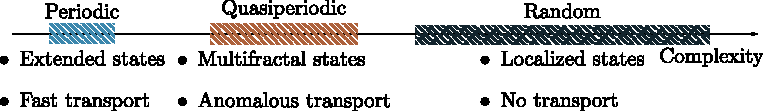
\includegraphics[width=0.5\textwidth]{img/1_motivation/complexity}

}

Cold atoms: \textbf{well-controlled} systems, strong \textbf{interactions}

\begin{columns}
\begin{column}{0.4\textwidth}
\centering
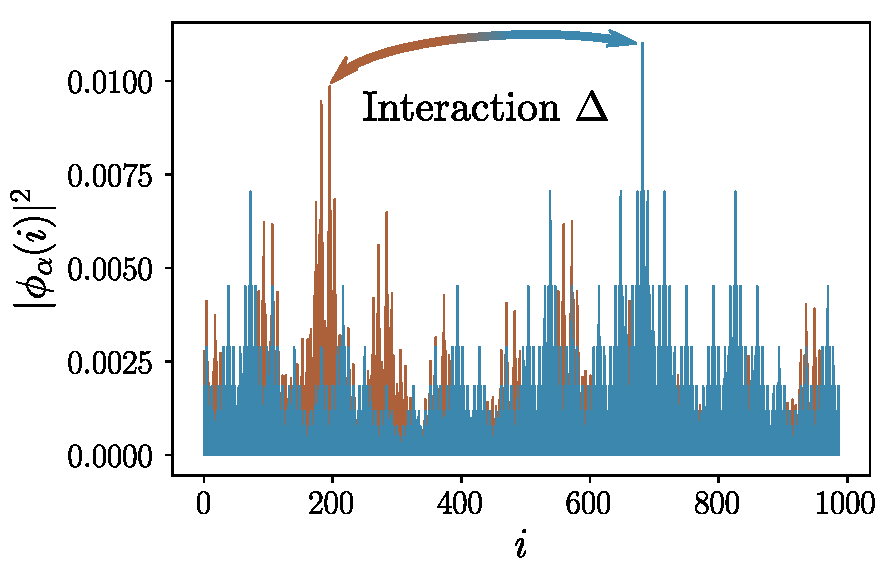
\includegraphics[height=3.5cm]{img/0_cover/free_two_densities_interaction}
\end{column}
\begin{column}{0.6\textwidth}
\textbf{Quasiperiodicity (QP) + strong interactions?}

Naively: delocalisation, fast transport

\textbf{Results}: 
\begin{itemize}
	\item weak QP: delocalisation, fast transport
	\item strong QP: \textbf{many-body localisation}, no transport
\end{itemize}
\end{column}
\end{columns}
\end{frame}

\begin{frame}{Outline}
\tableofcontents[hideallsubsections]
\end{frame}
\section{Many-body localisation}
\subsection{Dummy}
\begin{frame}{Many-body localisation}
\begin{block}{\textbf{Isolated} quantum system, \textbf{strong interactions}, disorder or quasiperiodicity}
	\begin{enumerate}
		\item Usual: ergodic dynamics, transport, \textcolor{comp}{eigenstate thermalisation hypothesis (ETH)},
		\item Unusual: non-ergodicity, no transport, \textcolor{BostonBlue}{many-body localisation (MBL)}.
	\end{enumerate}
\end{block}

\begin{columns}
\begin{column}{0.5\textwidth}
\centering
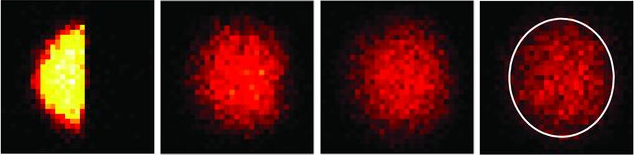
\includegraphics[width=0.9\columnwidth]{img/2_MBL/Imbalance_Choi_thermal}

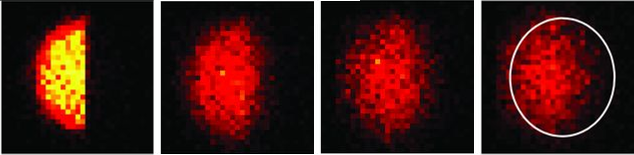
\includegraphics[width=0.9\columnwidth]{img/2_MBL/Imbalance_Choi}

[Choi \emph{et al} 16]
\end{column}
\begin{column}{0.5\textwidth}
\textbf{Experiments}: cold ions/atoms {\footnotesize[Schreiber \emph{et al} 15; Smith \emph{et al} 15; Bordia \emph{et al} 17]}.

\textbf{Motivations}:
\begin{itemize}
	\item ETH/MBL phase transition,
	\item MBL in more than 1D,
	\item Ingredients for MBL (this talk).
\end{itemize}
\end{column}
\end{columns}
\end{frame}

\begin{frame}{A model for MBL}
Chain of interacting spinless fermions (nb: no phonons):
\[
	H = \sum_{i=1}^L \left[ J (c_i^\dagger c_{i+1} + \text{h.c}) + \Delta n_i n_{i+1} - h_i n_i \right]
\]

\begin{columns}
\begin{column}{0.5\textwidth}
Disordered:
\centering
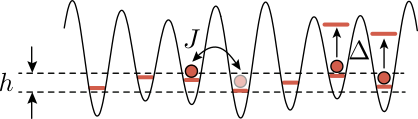
\includegraphics[height=2cm]{img/2_MBL/XXZ_cold_atoms}
\end{column}
%
\begin{column}{0.5\textwidth}
Quasiperiodic (this talk):
\centering
\includegraphics[height=2cm]{img/2_MBL/XXZ_QP_cold_atoms}
\end{column}
\end{columns}
Generic model: fermions, $\frac{1}{2}$ spins, hardcore bosons.

{
\centering

\includegraphics[width=0.5\textwidth]{img/2_MBL/arrow}

}
\end{frame}

\begin{frame}{MBL phenomenology}
\begin{columns}
\begin{column}{0.5\textwidth}
\centering
Phase diagram at $\Delta = 1$ {\footnotesize[Luitz \emph{et al} 15]}

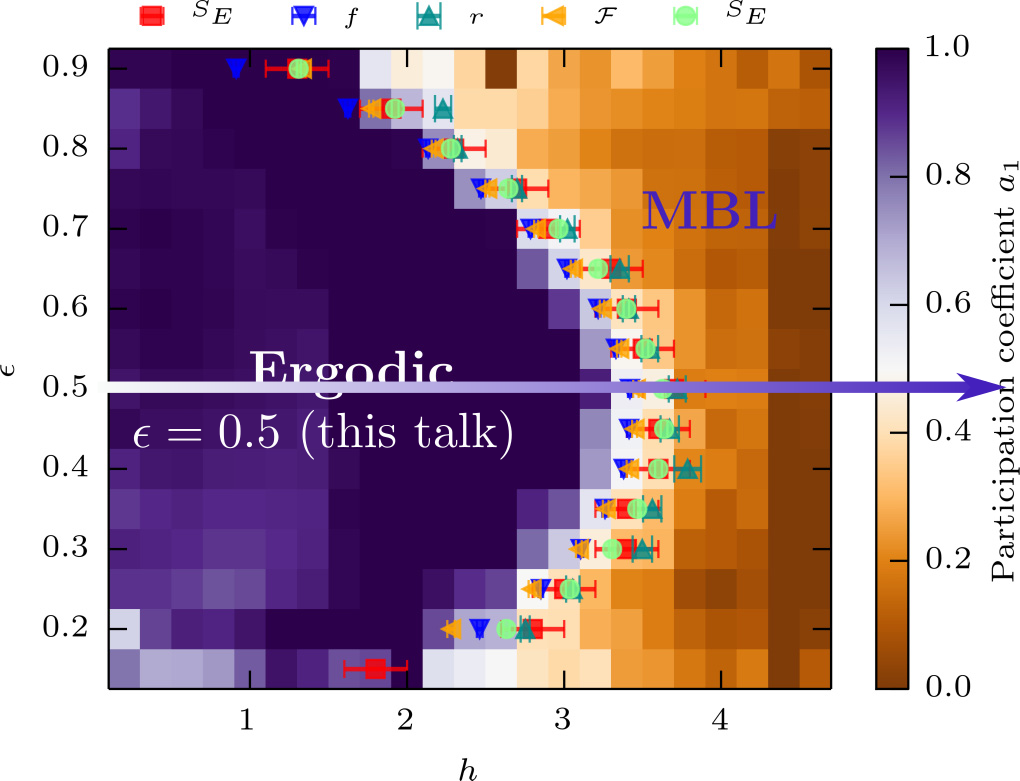
\includegraphics[width=0.75\textwidth]{img/2_MBL/edge2}
\end{column}
\begin{column}{0.5\textwidth}
\centering
Fermion density at $\epsilon = 0.5$
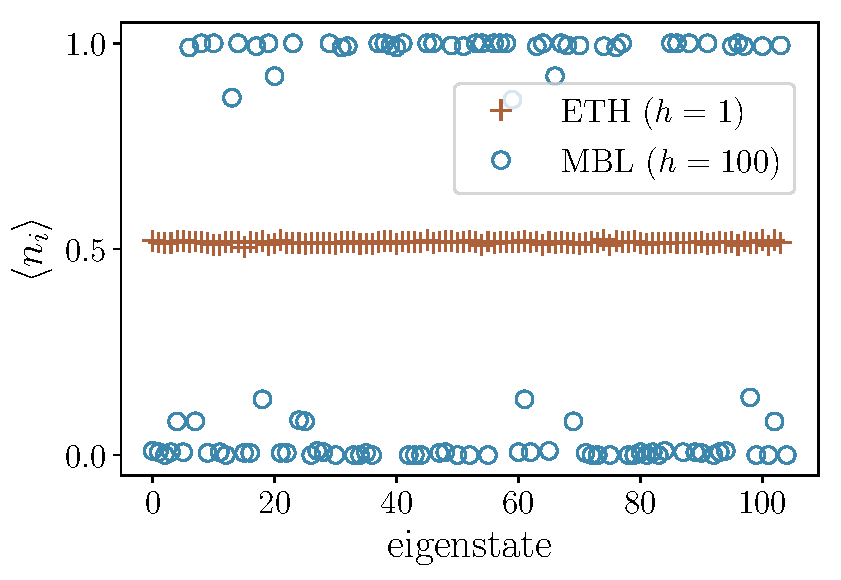
\includegraphics[width=0.8\textwidth]{img/2_MBL/local_observable}
\end{column}
\end{columns}
%%%%%%%%%%%%%%%%%%%%%%%%%%%%%%%%%%%%
\begin{columns}
\begin{column}{0.5\textwidth}
ETH:
\begin{itemize}
	\item Transport, thermal observables
	\item High entanglement
	\item Non-integrability
\end{itemize}
\end{column}
\begin{column}{0.5\textwidth}
MBL:
\begin{itemize}
	\item No transport, non-thermal observables
	\item Low entanglement
	\item Emergent integrability
\end{itemize}
\end{column}
\end{columns}
\end{frame}

\begin{frame}{Ingredients for MBL}
\begin{columns}
\begin{column}{0.65\textwidth}
Usually:
\begin{enumerate}
	\item $\Delta=0$: \textbf{localized} (random, Aubry-André potential)
	\item $\Delta \neq 0$: localization persists
\end{enumerate}
\end{column}
\begin{column}{0.35\textwidth}
\centering
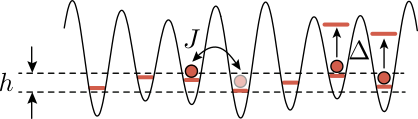
\includegraphics[width=\textwidth]{img/2_MBL/XXZ_cold_atoms}
\end{column}
\end{columns}
~\\
~\\

\begin{columns}
\begin{column}{0.65\textwidth}
This talk
\begin{enumerate}
	\item $\Delta=0$: \textbf{multifractal} (quasiperiodic potential)
	\item $\Delta\neq0$: localization appears
\end{enumerate}
\end{column}
\begin{column}{0.35\textwidth}
\centering
\includegraphics[width=\textwidth]{img/2_MBL/XXZ_QP_cold_atoms}
\end{column}
\end{columns}
~\\

\begin{block}{\textbf{Interest}}
\begin{itemize}
	\item MBL is \textbf{generic}
	\item Interplay between quasiperiodicity and MBL
\end{itemize}
\end{block}

\end{frame}
\section{Free Fibonacci chain at high energy}
\subsection{Dummy}
\begin{frame}{Interacting fermions on the Fibonacci chain}
\begin{columns}
\begin{column}{0.5\textwidth}
\centering
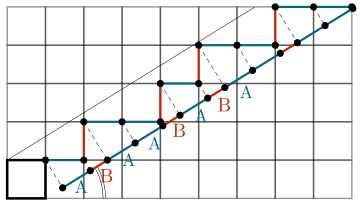
\includegraphics[width=0.8\textwidth]{img/3_Fibonacci/full_cp}
\end{column}
%%%%%%%%%%%%%
\begin{column}{0.5\textwidth}
\centering
\includegraphics[width=0.8\textwidth]{img/3_Fibonacci/XXZ_QP_cold_atoms}
\[
	H = \sum_{i=1}^L \left[ J (c_i^\dagger c_{i+1} + \text{h.c}) + \Delta n_i n_{i+1} - h_i n_i \right]
\]
\end{column}
\end{columns}
\begin{block}{Method: numerical \textbf{exact diagonalization}}
\begin{itemize}
	\item High energy + non-integrable: \textbf{no analytical methods}
	\item $L/2$ fermions on $L$ sites: $\# \text{states} \sim 2^L/\sqrt{L} \to$ \textbf{memory is limiting}

State-of-the art: $L=24$ {\footnotesize[Pietracaprina \emph{et al} 18]}

	\item Fibonacci: \textbf{few samples}: $L/2$ non-equivalent systems of size $L$.
\end{itemize}
\end{block}
\end{frame}

\begin{frame}{Free fermions properties}
\begin{itemize}
	\item Mutlifractal single particle wavefunctions {\footnotesize[Ostlund; Kalugin; Khomoto; \dots]}
	\item Anomalous transport {\footnotesize[Mayou; Schreiber; Varma \& Žnidarič; \dots]}
\end{itemize}
\begin{columns}
\begin{column}{0.5\textwidth}
\centering
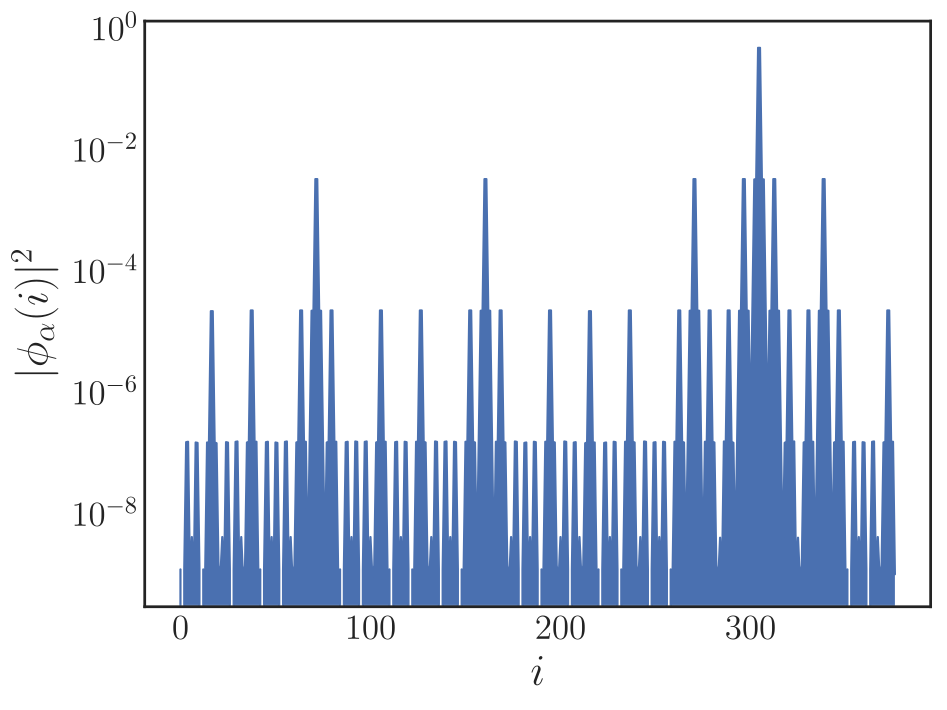
\includegraphics[width=0.8\textwidth]{img/3_Fibonacci/presence_prob}

{\footnotesize Single particle wavefunction at the Fermi level}
\end{column}
%%%%%%%%%%%%%%%%%%
\begin{column}{0.5\textwidth}
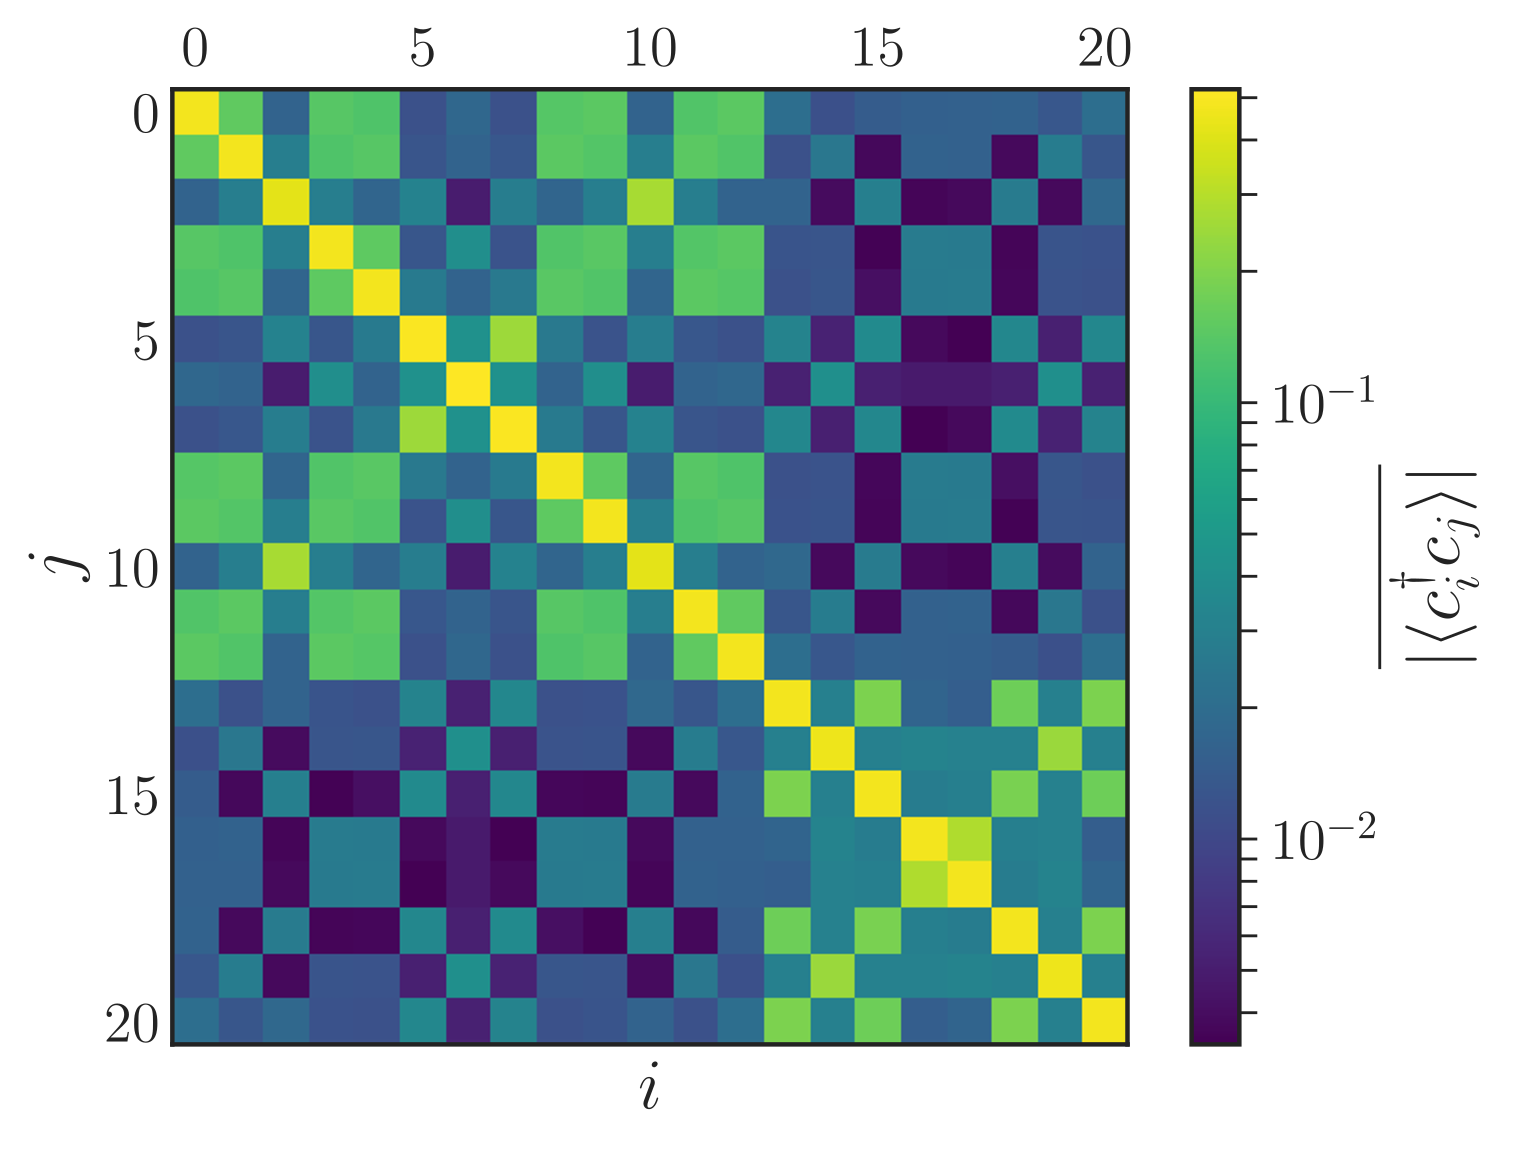
\includegraphics[width=0.8\textwidth]{img/3_Fibonacci/density_matrix_L21_h3}

{\footnotesize Correlations of highly excited states [Macé \emph{et al} 19]}
\end{column}
\end{columns}
\end{frame}

\begin{frame}{Free fermions entanglement}
\begin{block}{Entanglement entropy $S(\psi)$: a many-body \textbf{locality} probe}
\begin{itemize}
	\item $S(\psi) = \#\{\text{bits of information recoverable by local measurements}\}$
	\item $S(\psi)$ large: extended (entangled) state, $S(\psi)$ small: localized state.
\end{itemize}
\end{block}
%%%%%%%%%
\begin{columns}
\begin{column}{0.4\textwidth}
\centering
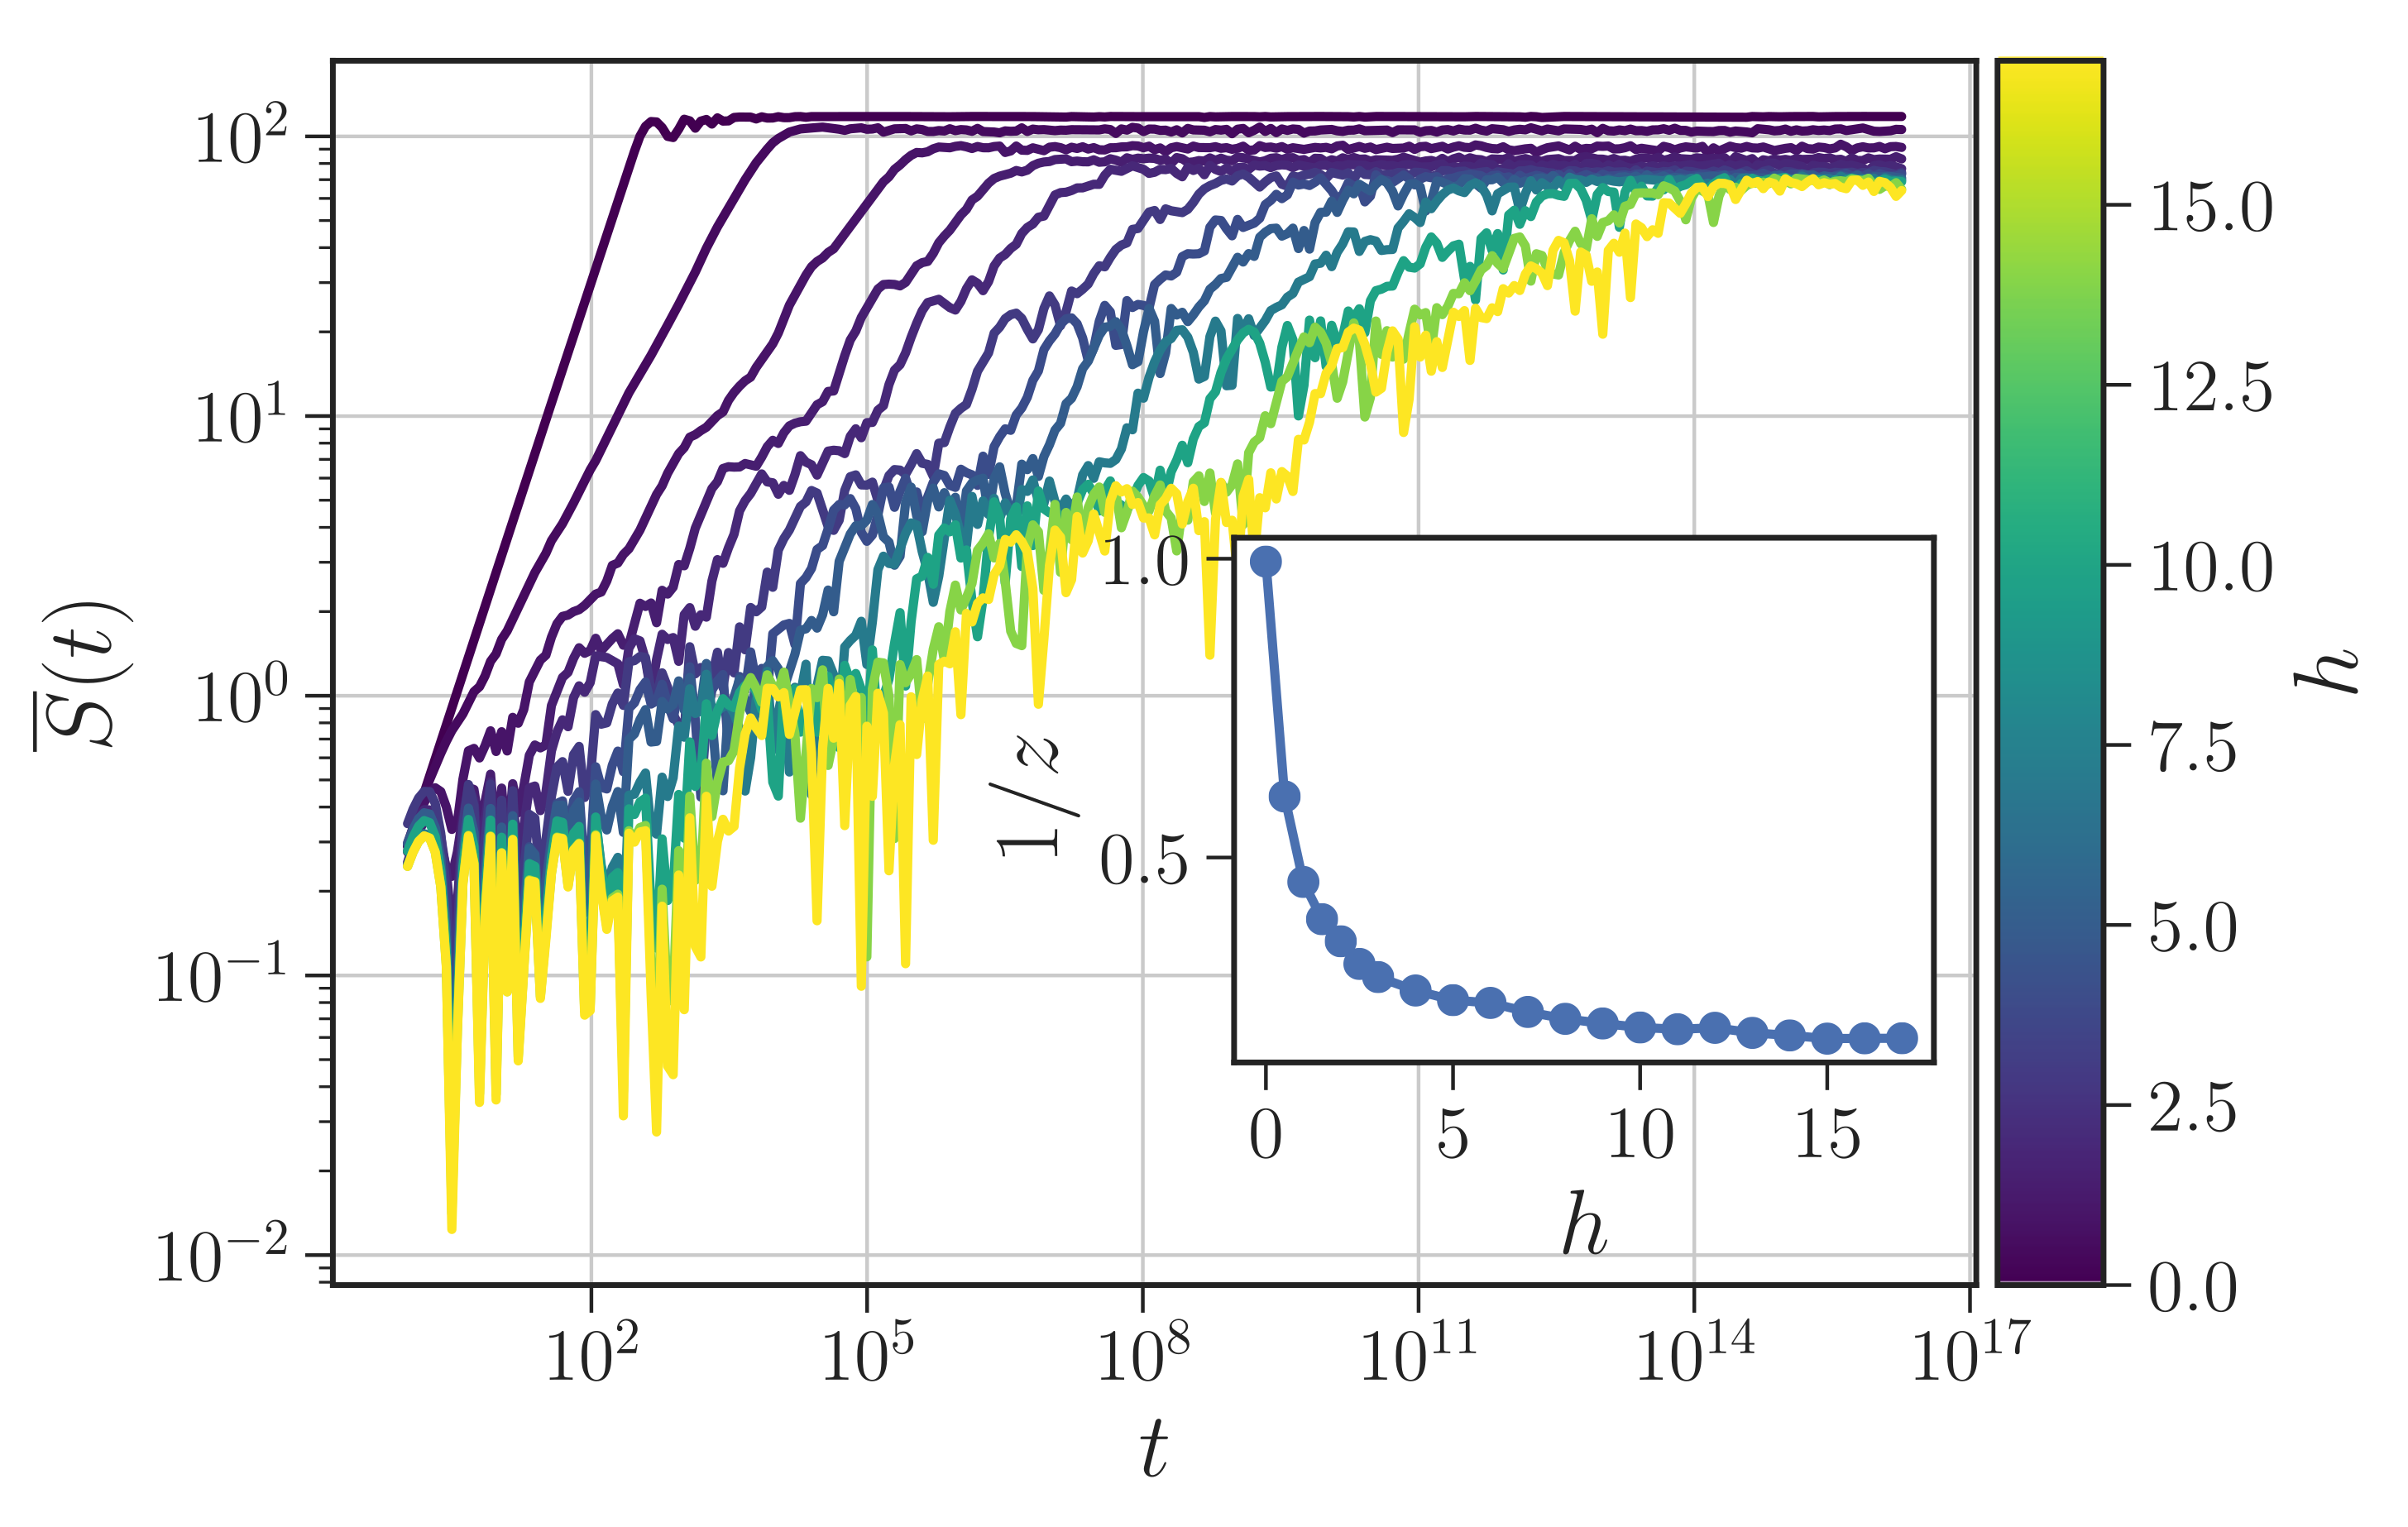
\includegraphics[width=\textwidth]{img/3_Fibonacci/free_fermions_entanglement_inset_coefficients}
{\footnotesize Entanglement growth starting from localized fermions [Macé \emph{et al} 19]}
\end{column}
%%%%%%%%%%%
\begin{column}{0.6\textwidth}
Fibonacci fermions: \textbf{anomalous} growth

$S(t) \sim t^{\frac{1}{z}},~z > 1$

Compare with:
\begin{itemize}
	\item Periodic system: $z=1$ (ballistic growth),
	\item Disordered system: $z \to \infty$ (no growth).
\end{itemize}
\begin{block}{\textbf{Conclusion}}
Anomalous, intermediate prop.\, even at high energy.
\end{block}
\end{column}
\end{columns}
\end{frame}

\section{Interacting Fibonacci chain}
\subsection{Dummy}
\begin{frame}{The ETH/MBL transition: 1) spectral properties}
\begin{columns}
\begin{column}{0.5\textwidth}
Gap ratios {\footnotesize [Oganesian, Huse]}
\[
	r_n = \min\left(\frac{g_{n+1}}{g_n}, \frac{g_n}{g_{n+1}}\right)
\]
\begin{itemize}
	\item \textcolor{comp}{ETH: random matrix-like spectrum}
	$\overline{r}_\text{ETH} \simeq 0.53$
	\item \textcolor{BostonBlue}{MBL: independant levels}
	
	$\overline{r}_\text{MBL} \simeq 0.39$
\end{itemize}
\end{column}
%%%%%%%%%%%%%%%
\begin{column}{0.5\textwidth}
\centering
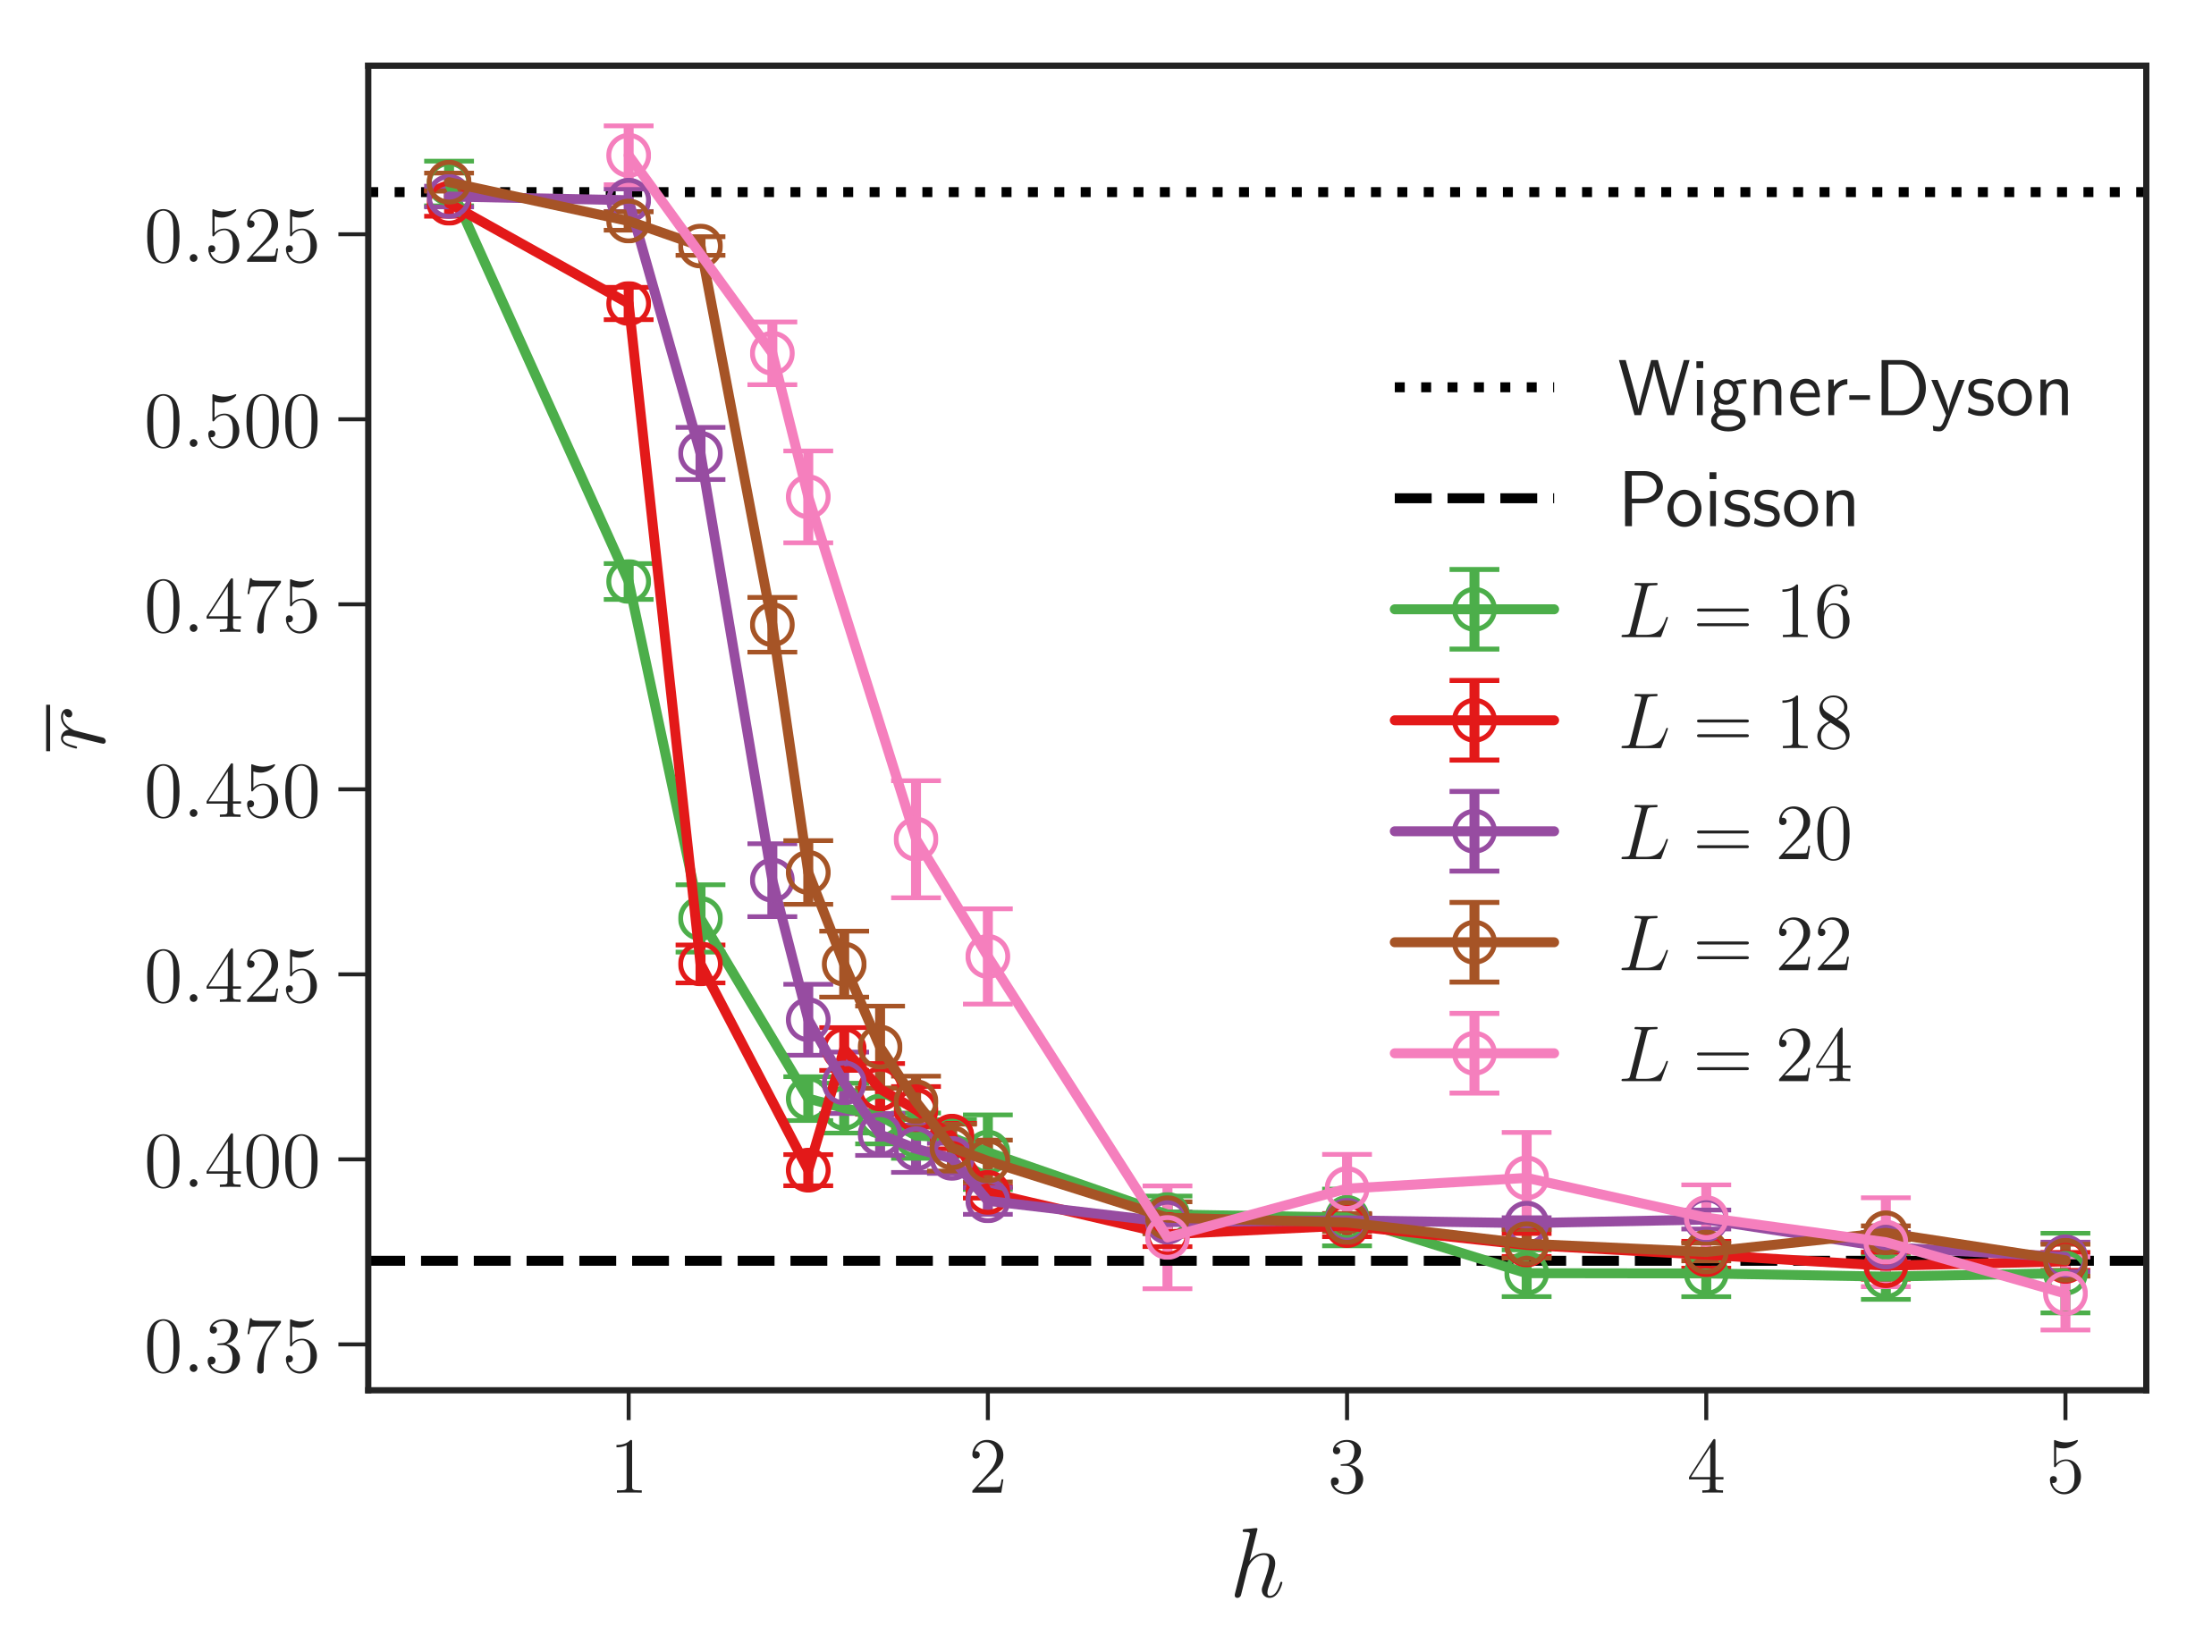
\includegraphics[width=0.9\textwidth]{img/3_Fibonacci/rgap}

Compatible with \textbf{ETH/MBL transition}, $h^* \simeq 2.5$.
\end{column}
\end{columns}
\end{frame}

\begin{frame}{The ETH/MBL transition: 2) Entanglement}
\begin{columns}
\begin{column}{0.5\textwidth}
Entanglement entropy:
\begin{itemize}
	\item \textcolor{comp}{ETH: coincides with thermodynamic entropy: \textbf{extensive}}
	
	$\overline{S}_\text{ETH} \simeq L$
	\item \textcolor{BostonBlue}{MBL: \textbf{sub-extensive}}
	
	$\overline{S}_\text{MBL}/L \to 0$
\end{itemize}
\end{column}
%%%%%%%%%%%%%%%
\begin{column}{0.5\textwidth}
\centering
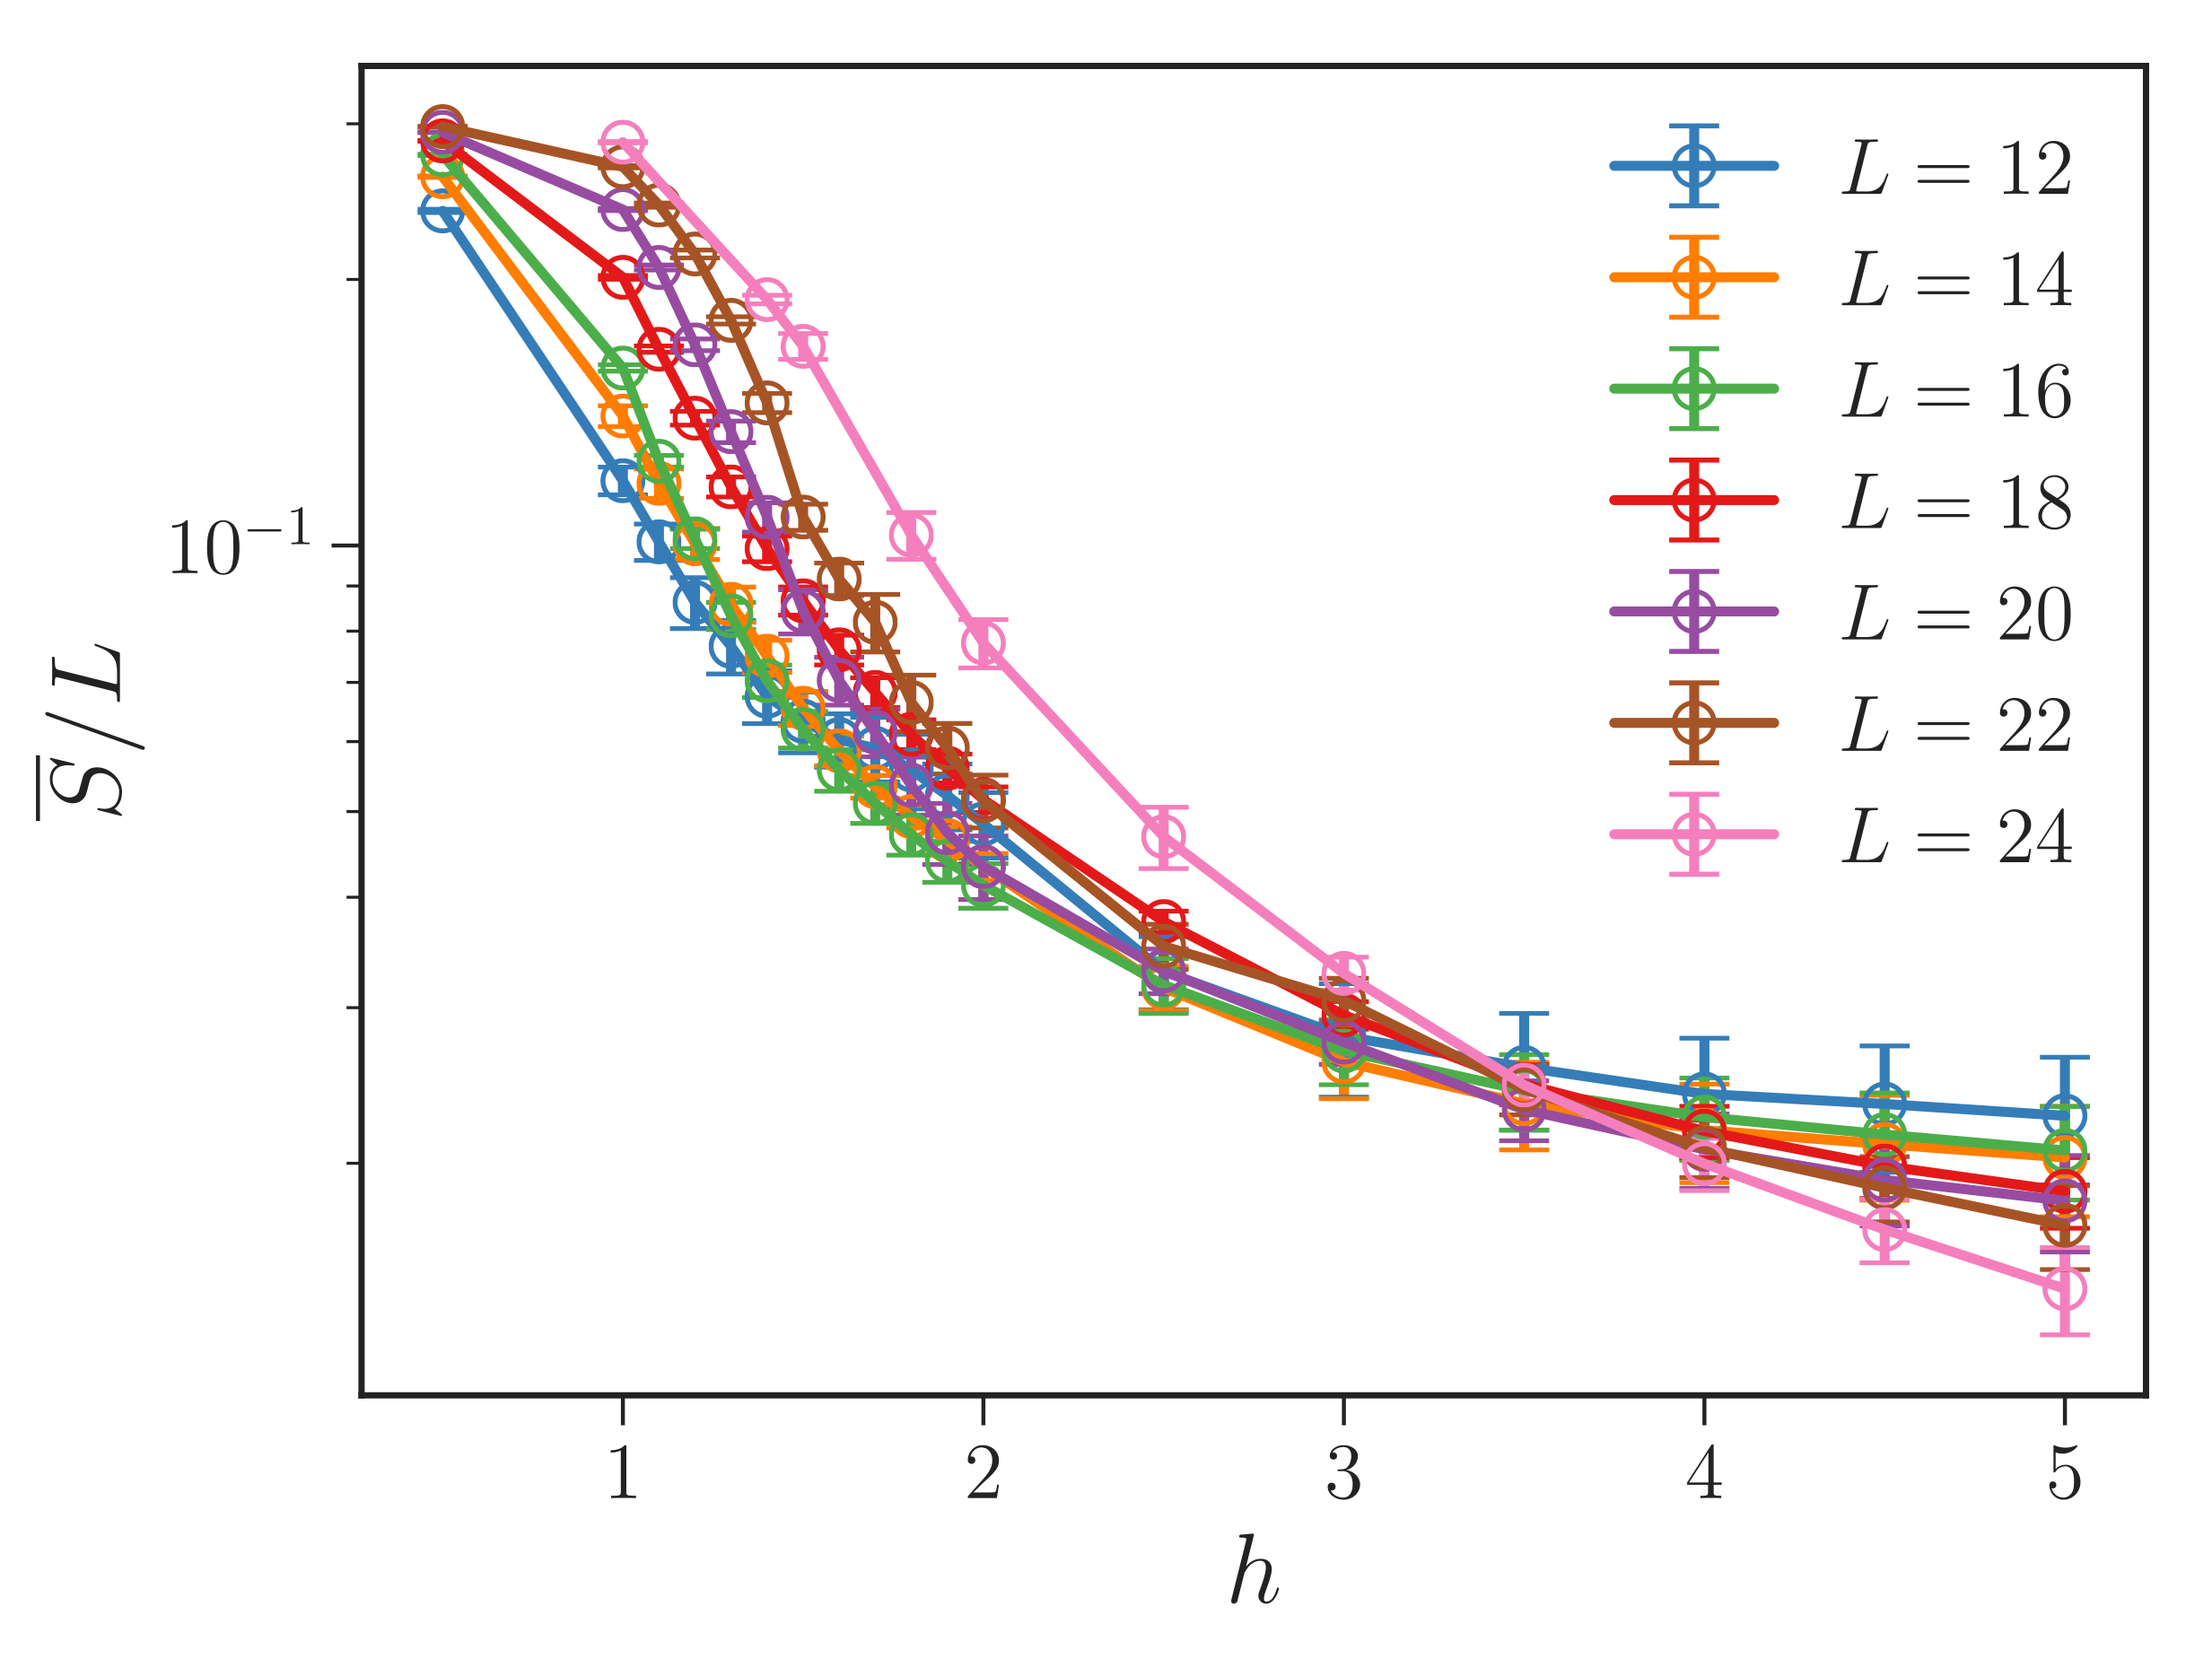
\includegraphics[width=0.9\textwidth]{img/3_Fibonacci/entropy}

Compatible with \textbf{ETH/MBL transition}, $h^* \simeq 3.5$.
\end{column}
\end{columns}
\end{frame}

\begin{frame}{The ETH/MBL transition: 3) Local observables}
Expect: \textcolor{comp}{$\langle n_i \rangle_\text{ETH} = \frac{1}{2}$}, \textcolor{BostonBlue}{$\langle n_i \rangle_\text{MBL} \simeq 0 \text{ or } 1$}.
\begin{columns}
\begin{column}{0.33\textwidth}
\centering
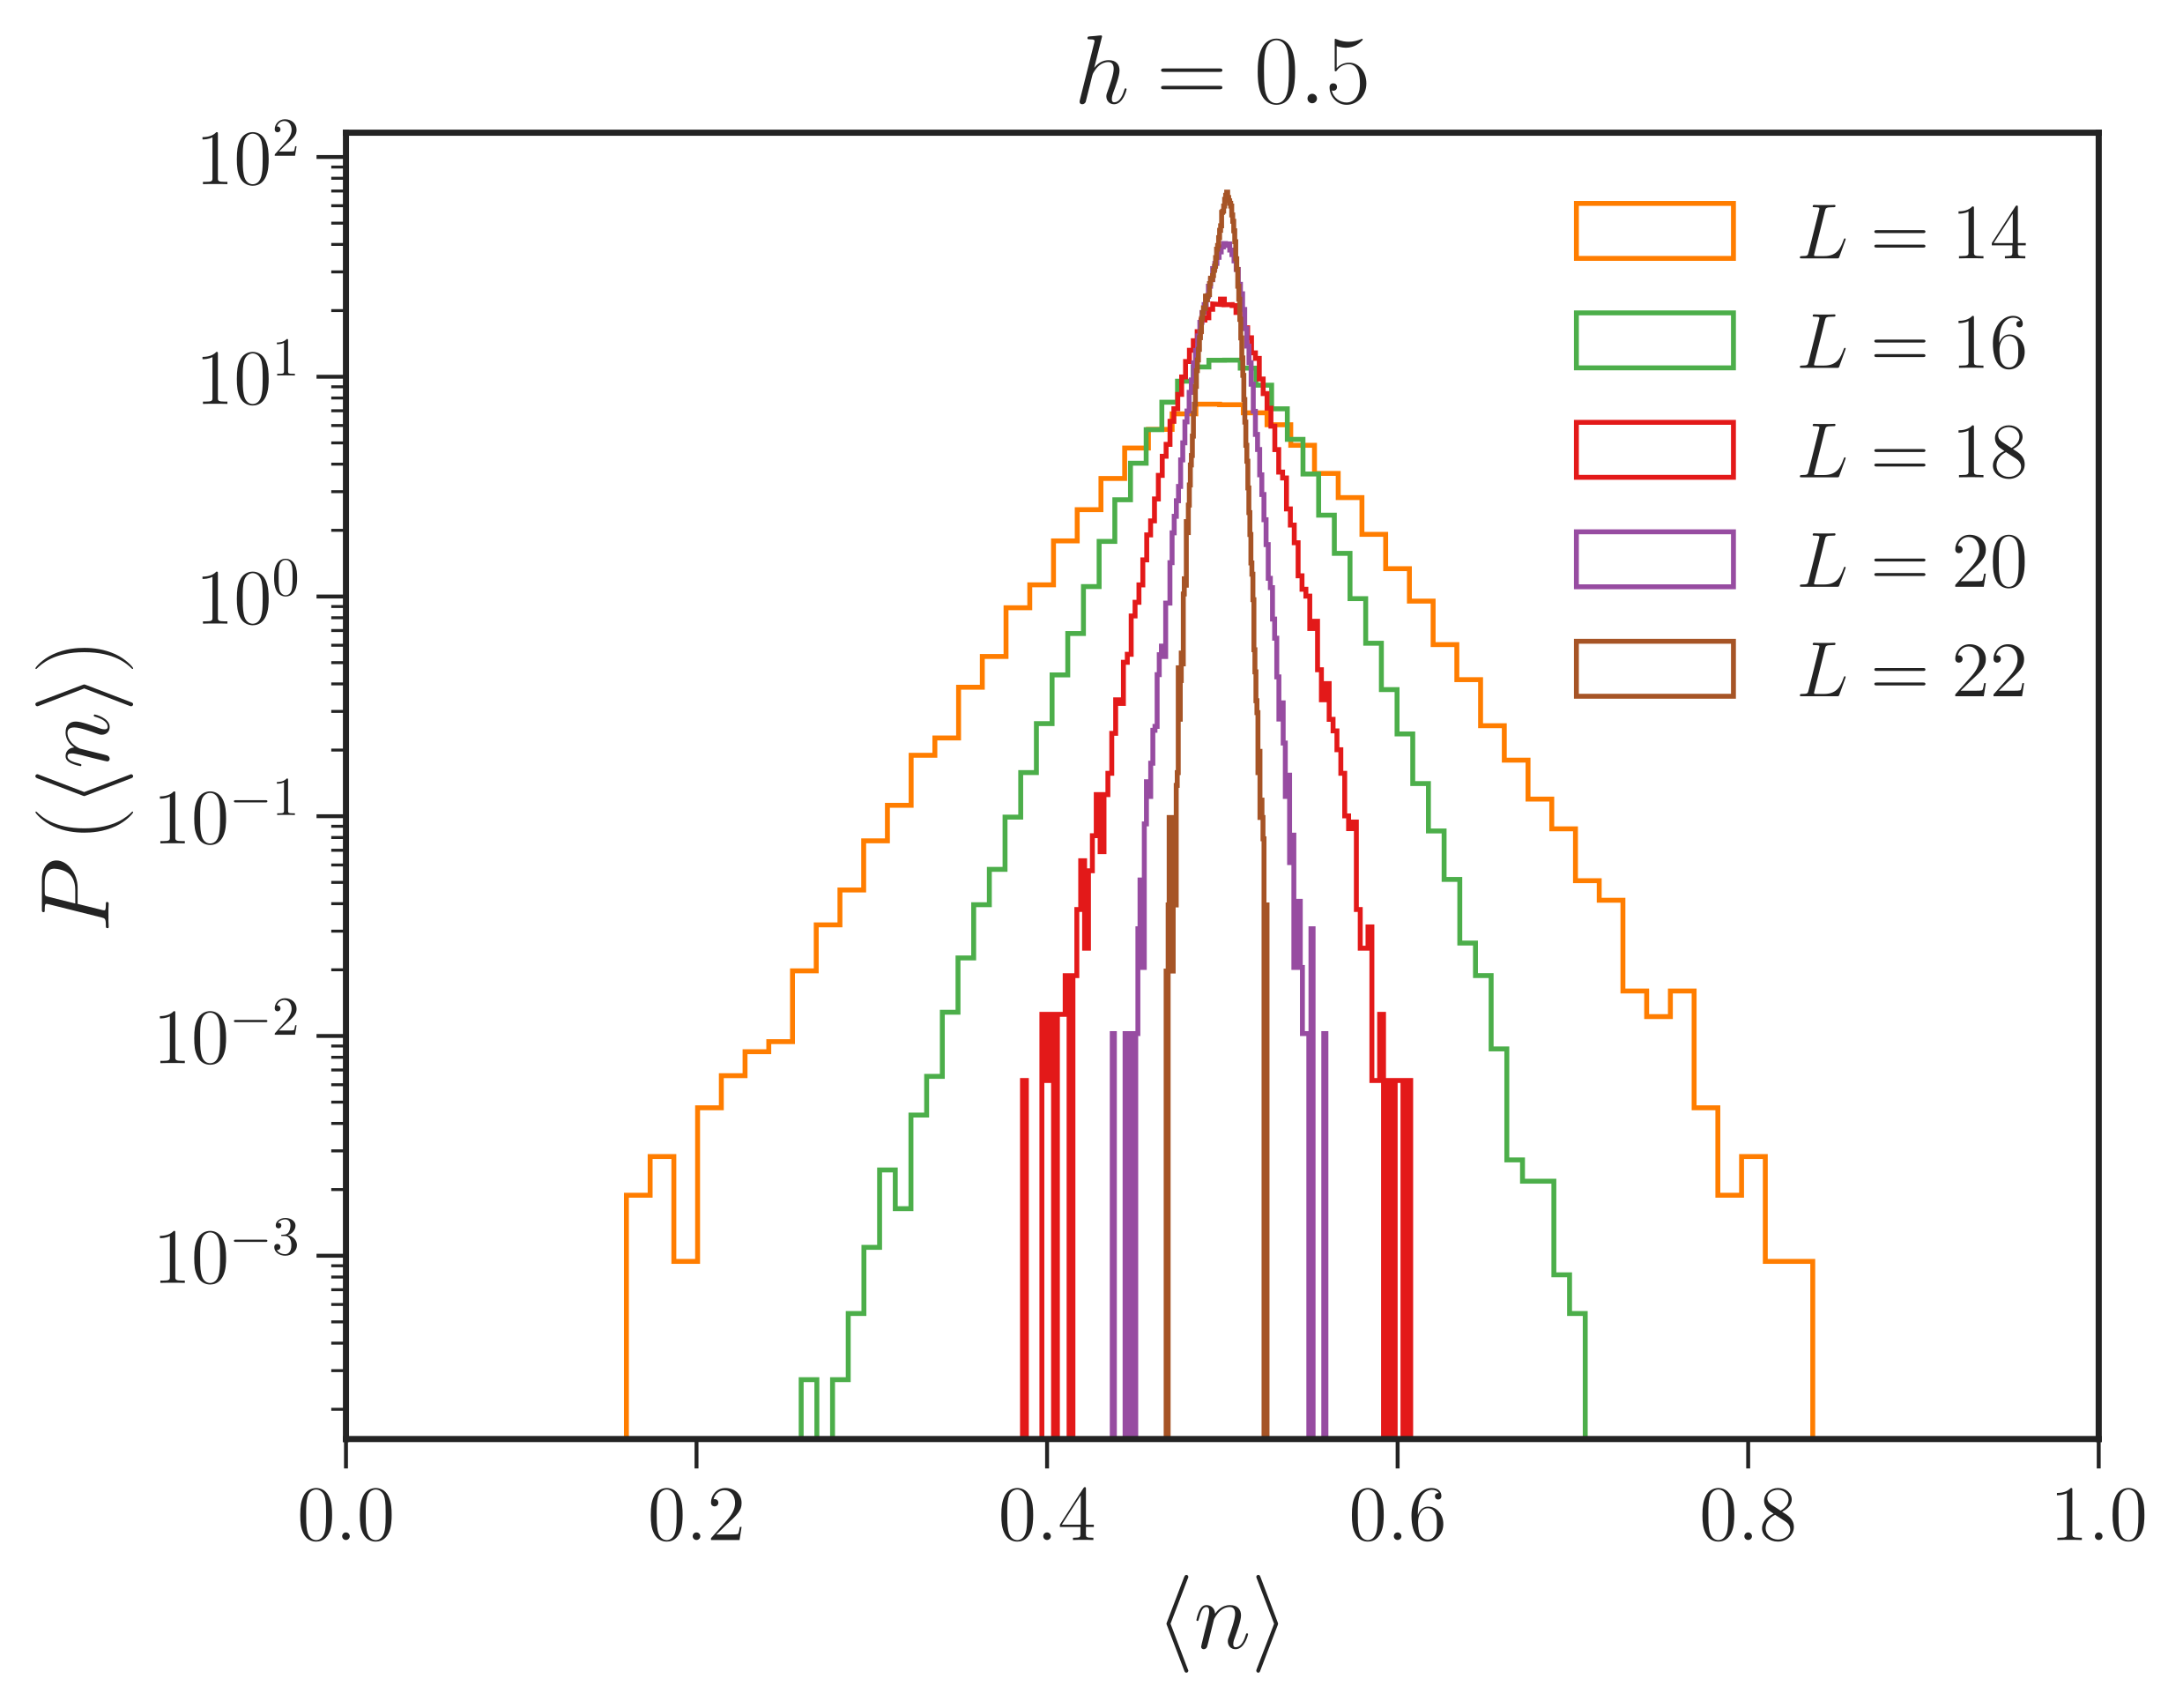
\includegraphics[width=\textwidth]{img/3_Fibonacci/sz_ETH}
{\footnotesize ETH Fibonacci}
\end{column}
%%%%%%%%%%
\begin{column}{0.33\textwidth}
\centering
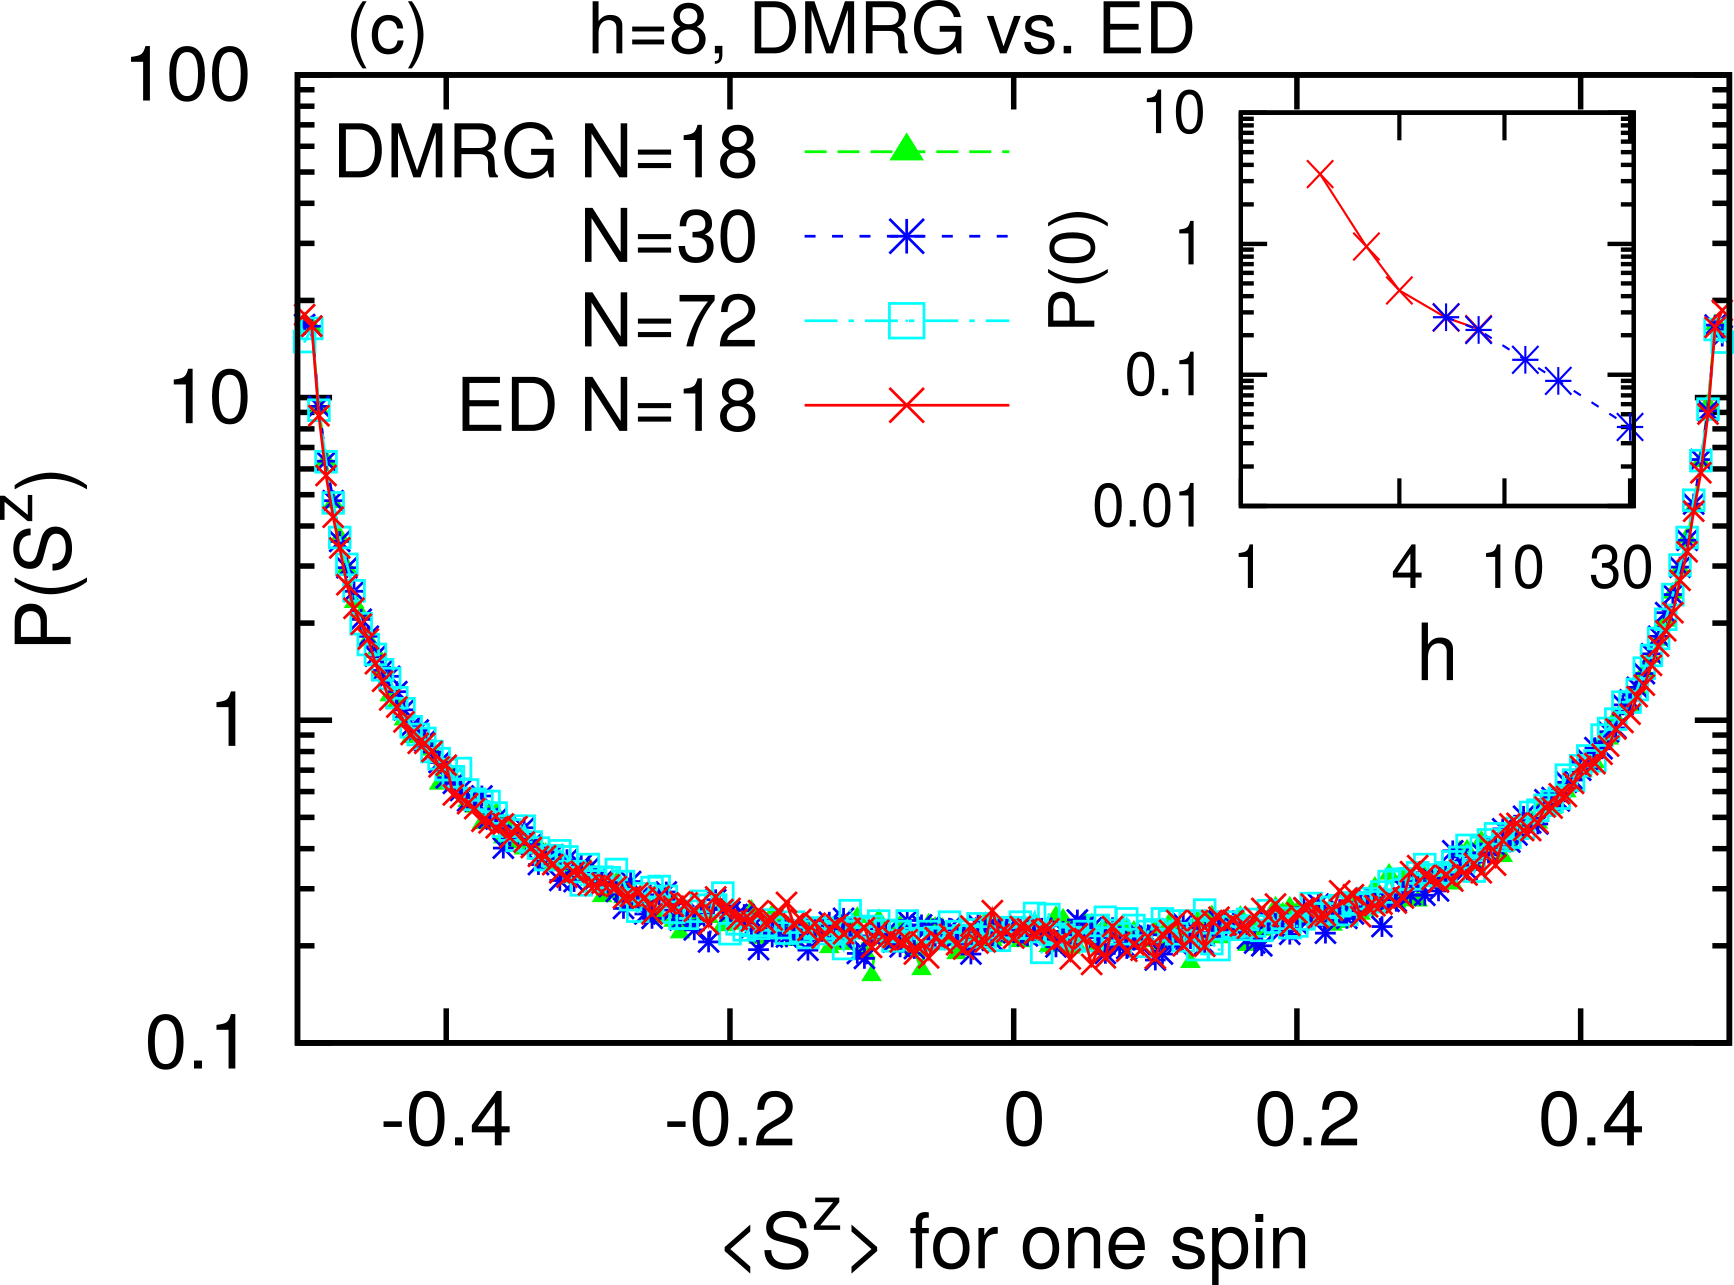
\includegraphics[width=\textwidth]{img/3_Fibonacci/surface768}
{\footnotesize MBL random [Lim, Sheng 15]}
\end{column}
%%%%%%%%%%
\begin{column}{0.33\textwidth}
\centering
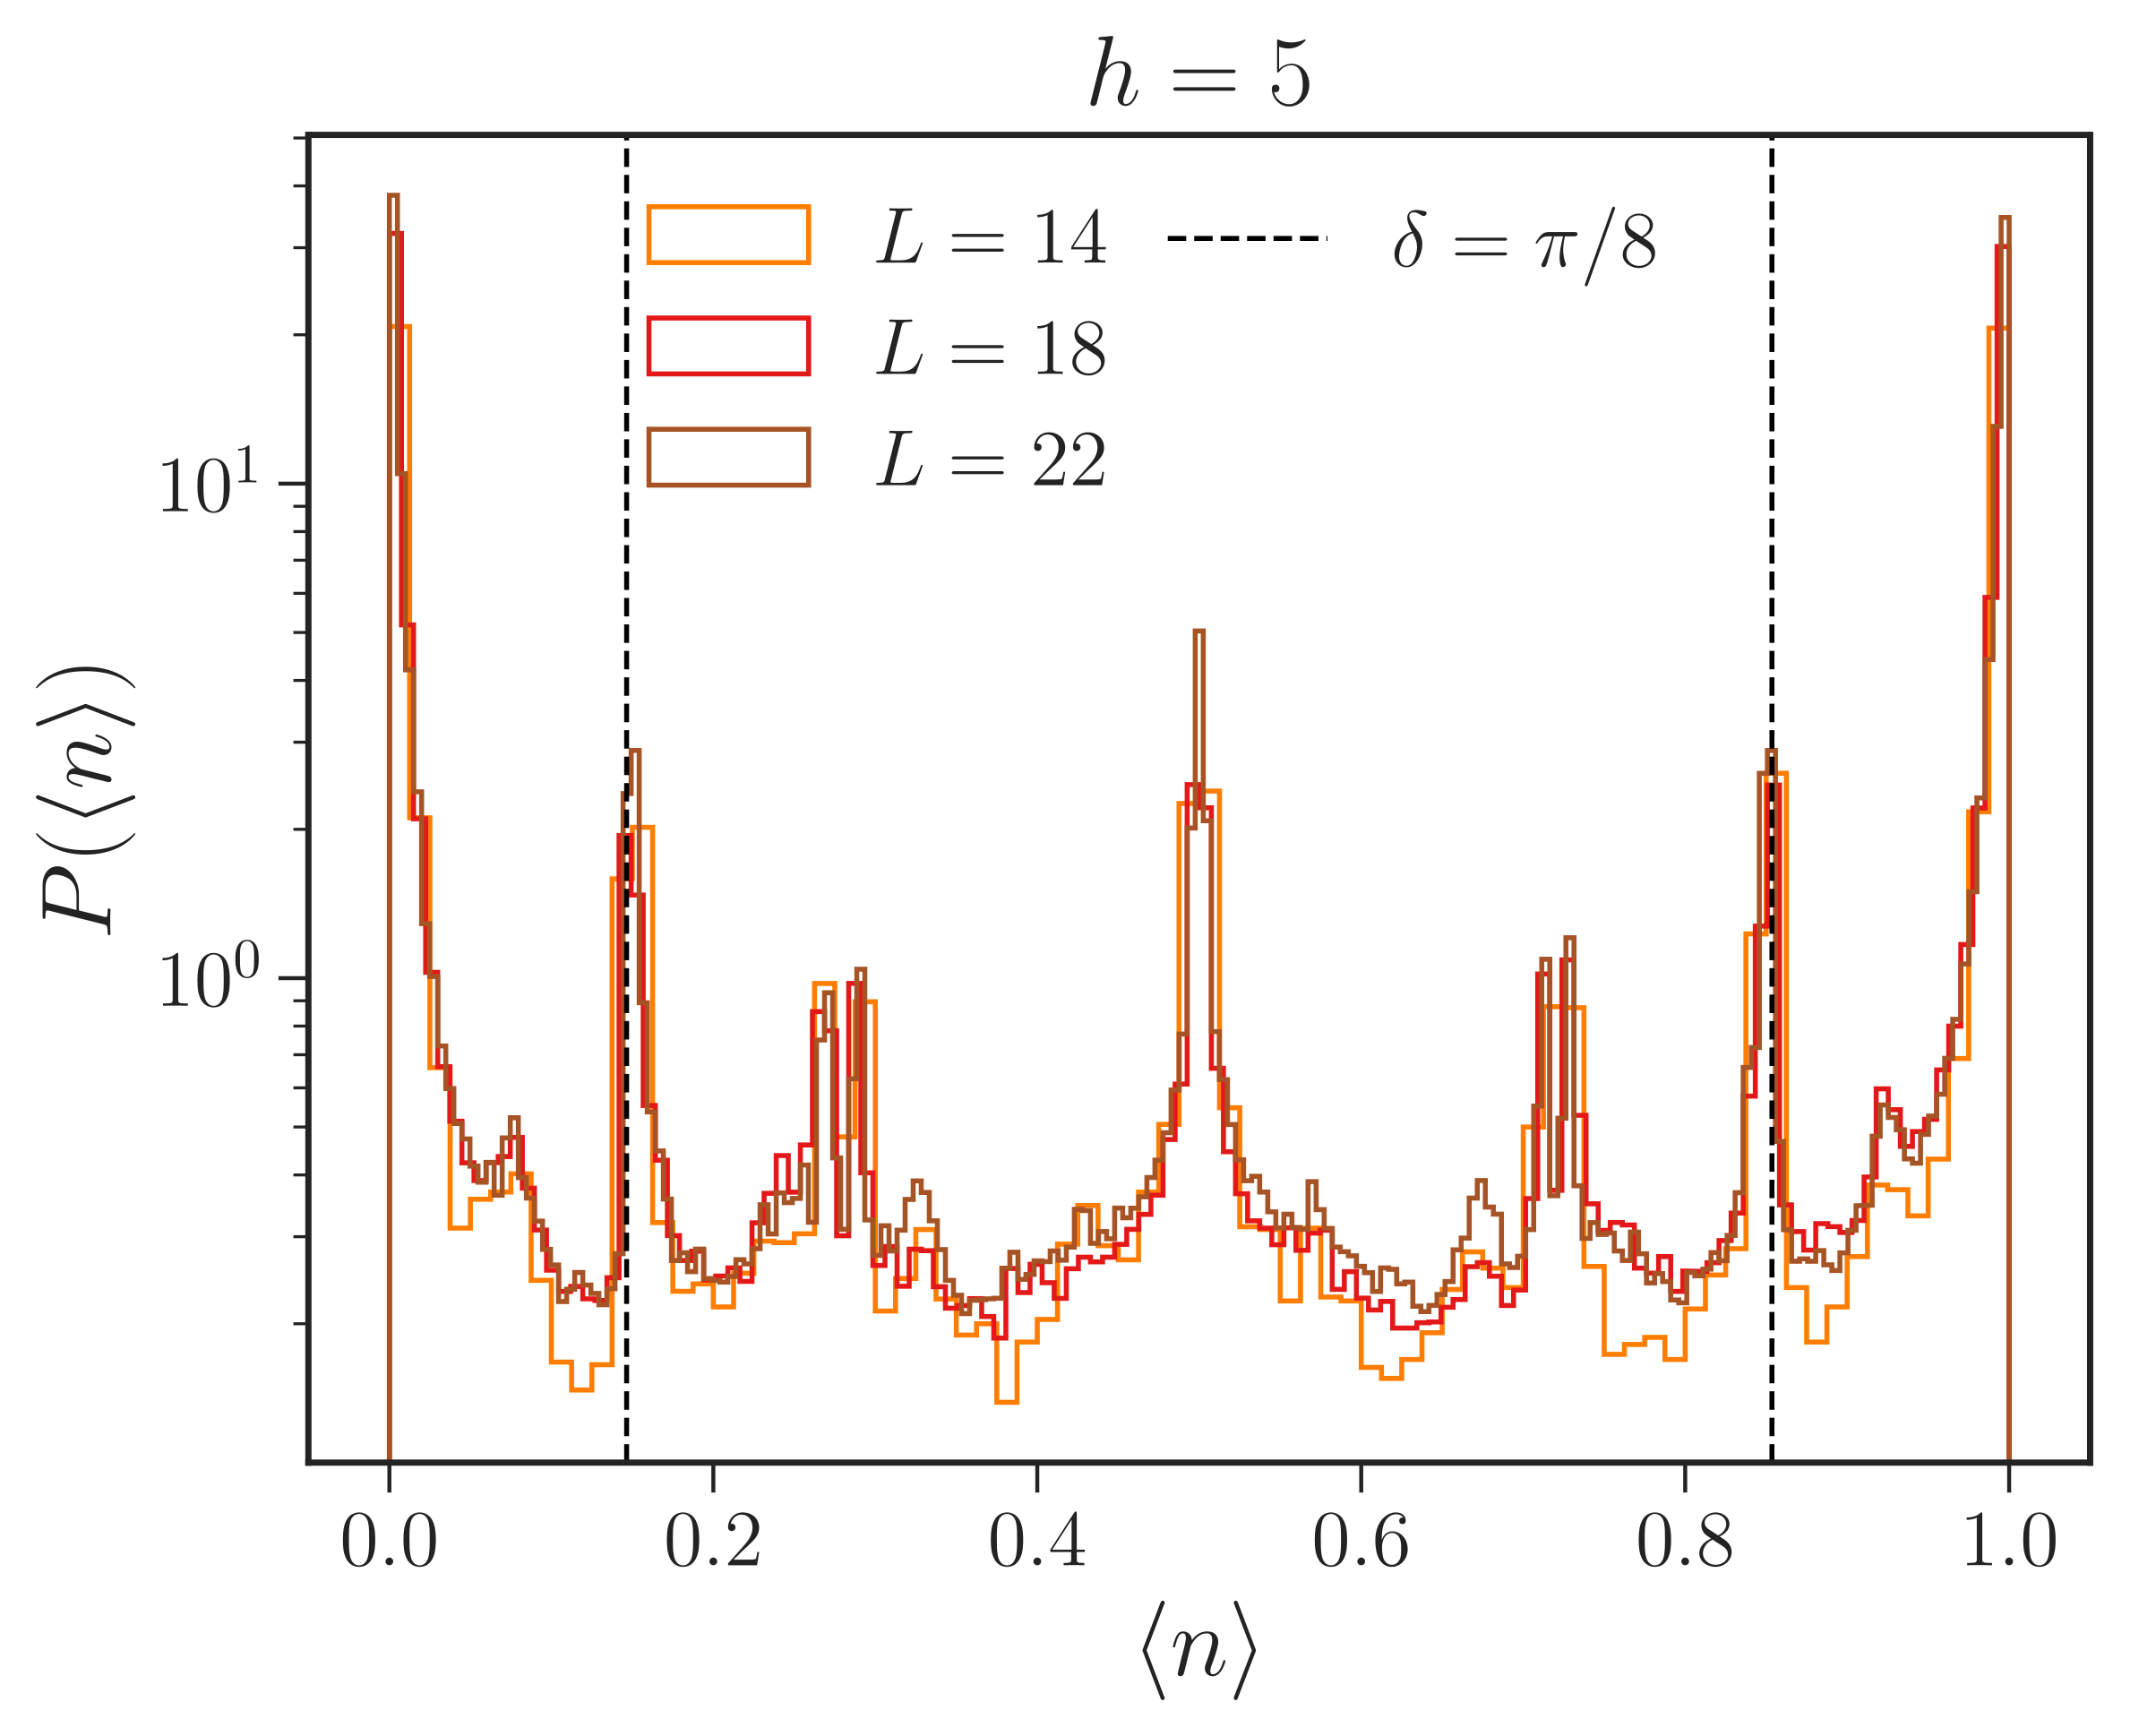
\includegraphics[width=\textwidth]{img/3_Fibonacci/sz_MBL}
{\footnotesize MBL Fibonacci}
\end{column}
%%%%%%%%%%
\end{columns}
~\\
~\\

Fibonacci MBL: \textbf{extra structure} $\to$ link with QP geometry?
\end{frame}

\begin{frame}{Fibonacci MBL: local entanglement}
\begin{columns}
\begin{column}{0.5\textwidth}
\centering
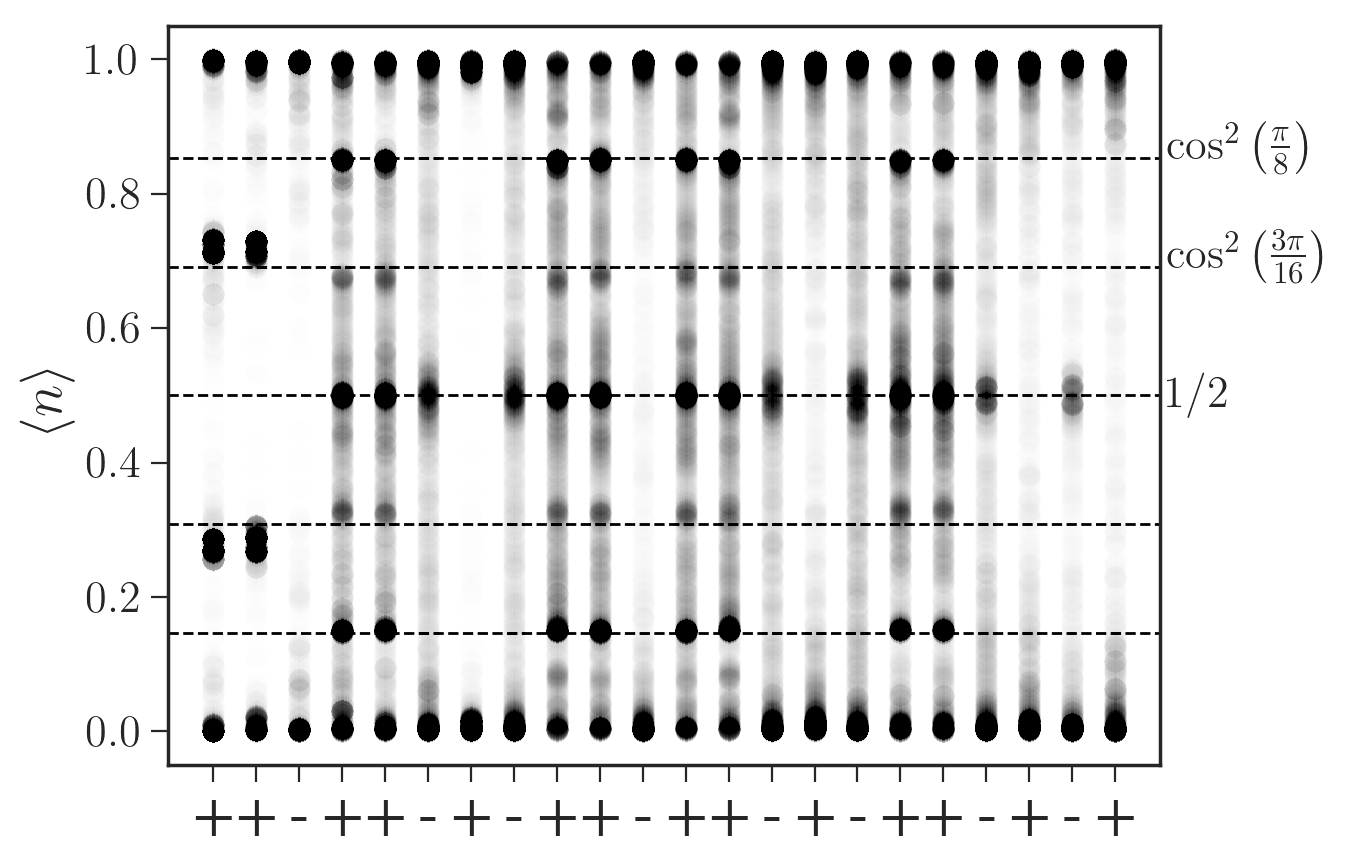
\includegraphics[width=0.8\textwidth]{img/3_Fibonacci/realspace_sz_L22_h5_shift1}
\end{column}
%%%%%%%%%%%%
\begin{column}{0.5\textwidth}
Density peaks on \textbf{AA pairs}

$\to$ 4 sites toy model BAAB

$\to$ locally entangled states

$\ket{\psi} = \cos \delta \ket{01} \pm \sin \delta \ket{10}$

with $\delta = 0,~\frac{\pi}{4},~\frac{\pi}{8}$.
\end{column}
\end{columns}
%%%%%%%%%%%%%%%%%%%%%%%%%%%%%%%
\begin{columns}
\begin{column}{0.33\textwidth}
\centering
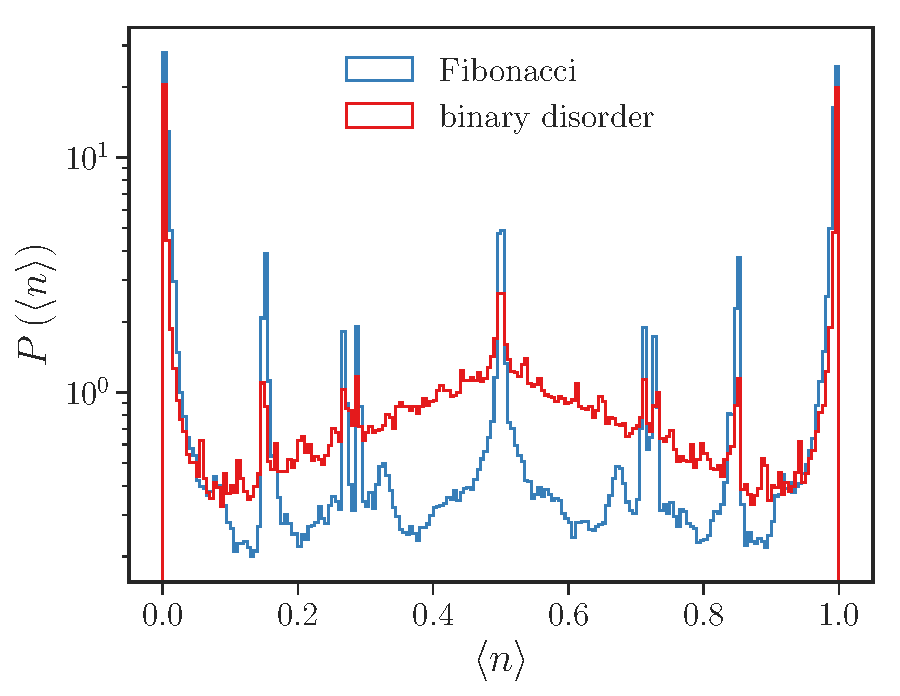
\includegraphics[width=0.8\textwidth]{img/3_Fibonacci/local_observable_fibo_shuffle_p_8_h_5_L_22}
\end{column}
%%%%%%%%%%%%
\begin{column}{0.33\textwidth}
Peak ingredients:
\begin{itemize}
	\item \textbf{Binary} modulation A/B
	\item \textbf{Correlated} modulation (Fibonacci)
\end{itemize}
\end{column}
%%%%%%%%%%%%
\begin{column}{0.33\textwidth}
\centering
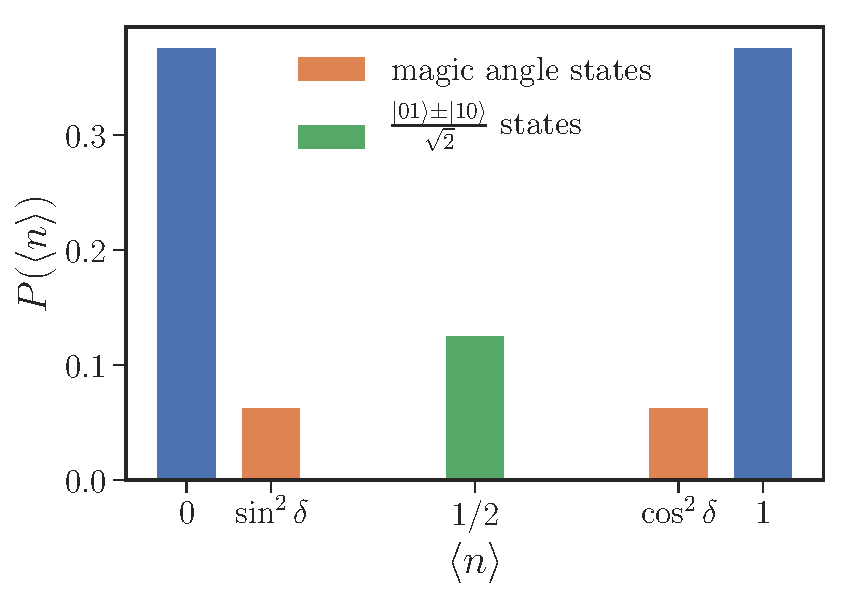
\includegraphics[width=0.8\textwidth]{img/3_Fibonacci/sz_perturbation_theory}
\end{column}
\end{columns}
\end{frame}

\begin{frame}{Dynamics: Imbalance}
\begin{columns}
\begin{column}{0.5\textwidth}
Imbalance experiment:
\begin{itemize}
	\item $\ket{\psi(t=0)}$: high energy product state
	\item Imbalance: \textbf{distance} from initial state
	
	$I(t) = \frac{4}{L}\sum_i \left\langle \left(n_i(t) - \frac{1}{2}\right)\left(n_i(0) - \frac{1}{2}\right) \right\rangle$
\end{itemize}

Properties:
\begin{itemize}
	\item \textcolor{comp}{ETH: power-law decay} $I(t) \sim t^{-\zeta}$
	\item \textcolor{BostonBlue}{MBL: saturation} $I(t\to \infty) = \text{cst} > 0$ 
	
	$\to$ \textbf{memory} of the initial state
	
	{\footnotesize [Luitz \emph{et at} 15]}
\end{itemize}
\end{column}
%%%%%%%%%%%%%%%%
\begin{column}{0.5\textwidth}
\centering
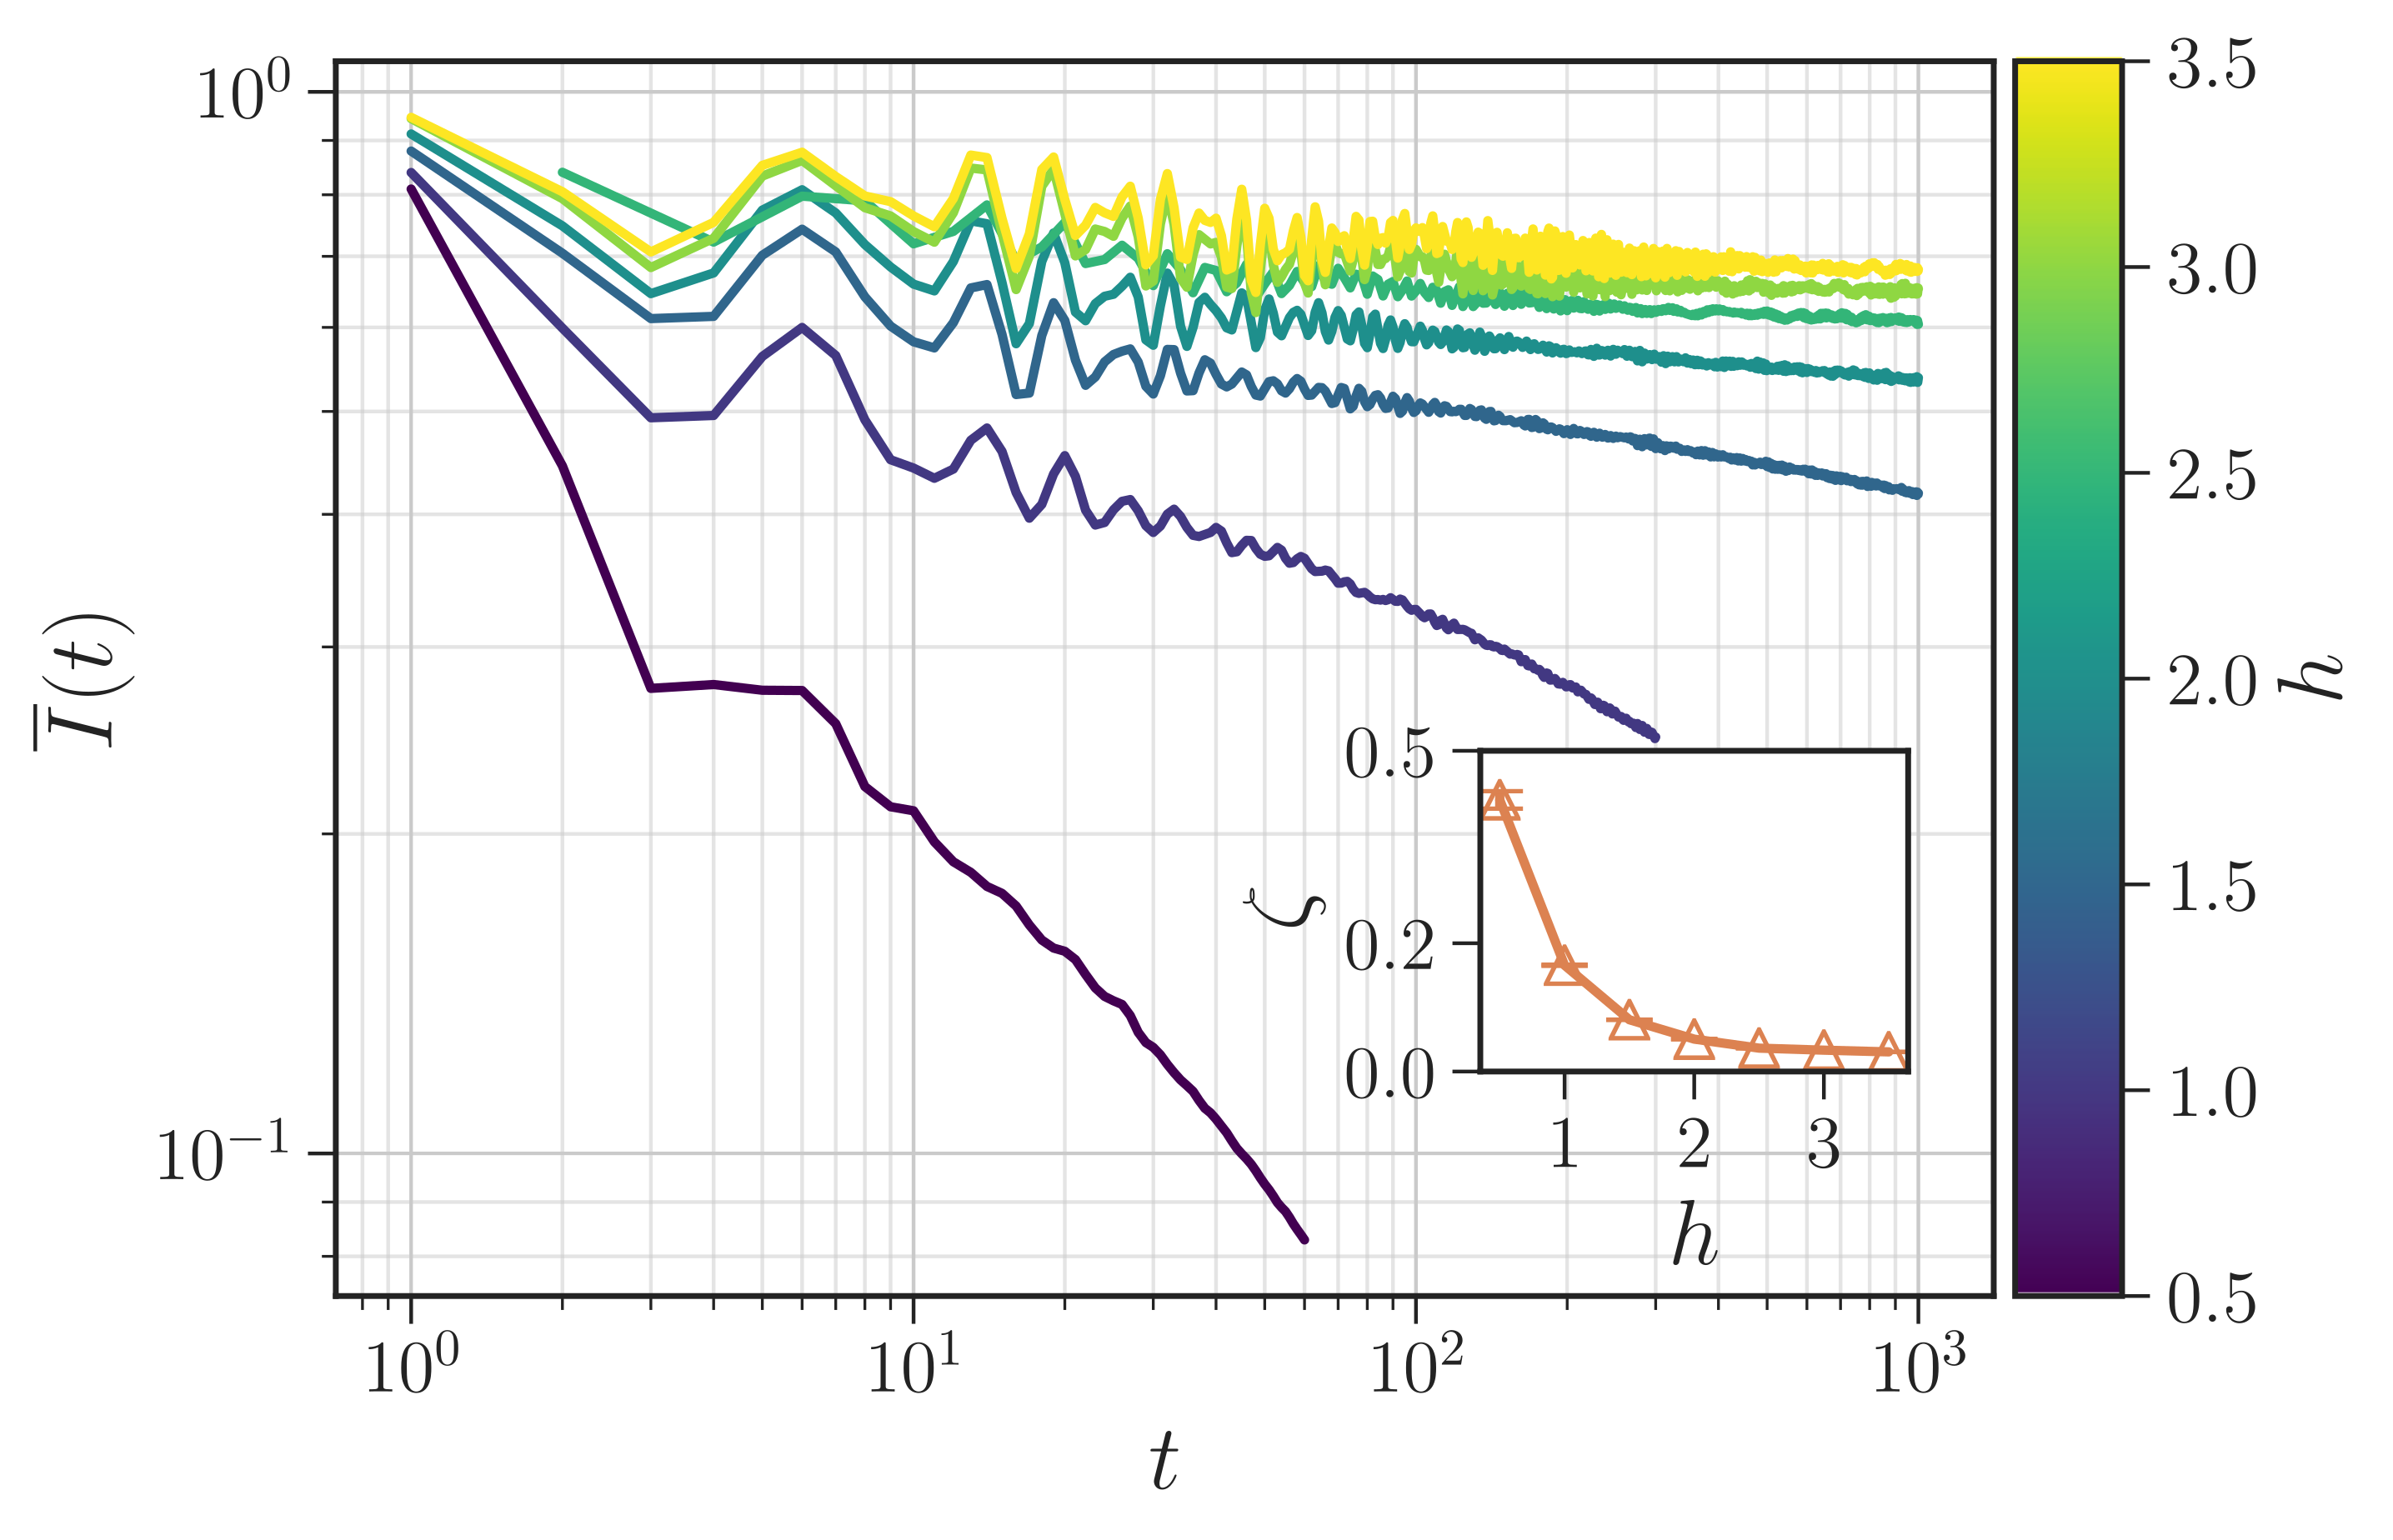
\includegraphics[width=\textwidth]{img/3_Fibonacci/imbalance}

$\zeta(h \geq 2.5) = 0 \to$ MBL phase transition.
\end{column}
%%%%%%%%%%%%%%%%
\end{columns}
\end{frame}

\begin{frame}{Dynamics: entanglement}
\textcolor{comp}{ETH phase}: expect $S(t) \propto t$

Fibonacci: \textbf{anomalous} $S(t) \propto t^{1/z}$, $z > 1$.

\begin{columns}
\begin{column}{0.5\textwidth}
\centering
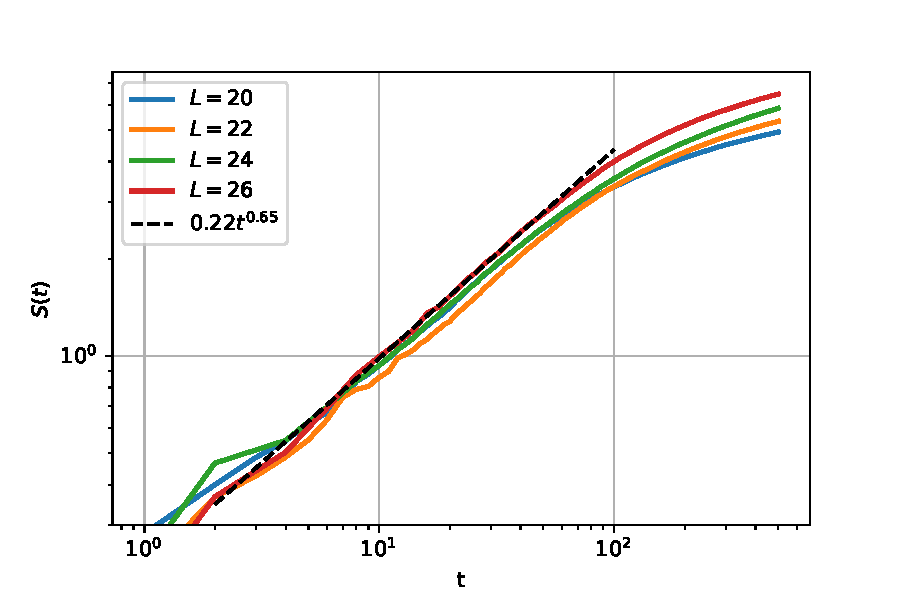
\includegraphics[width=0.8\textwidth]{img/3_Fibonacci/entanglement_scaling_h1_shift0}
\end{column}
%%%%%%%%%%%%%
\begin{column}{0.5\textwidth}
\centering
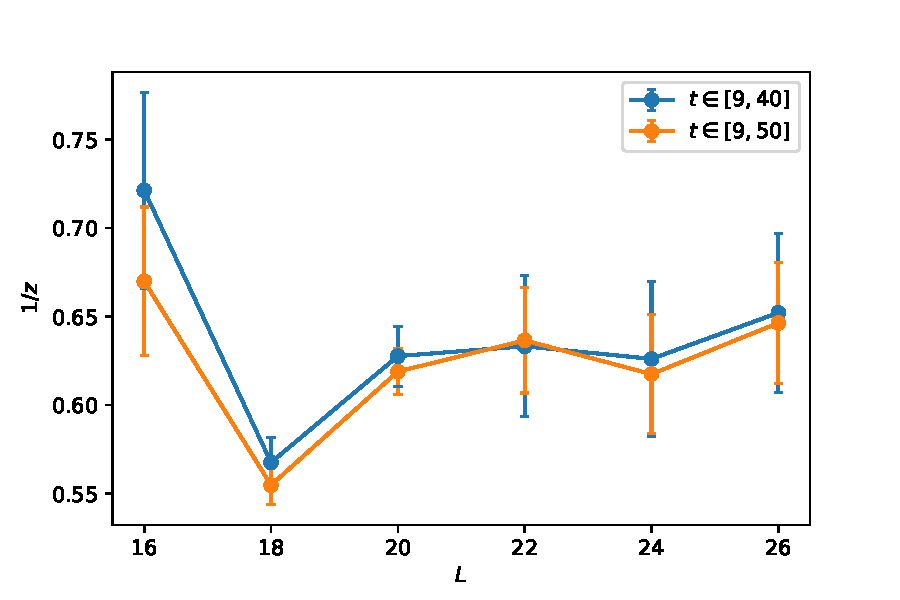
\includegraphics[width=0.8\textwidth]{img/3_Fibonacci/fits_entropy_h1_shift0}
\end{column}
\end{columns}
Usual explanation: \textbf{rare regions} {\footnotesize[Vosk; Potter 15]}

Fibonacci: no rare regions \dots 

Finite size effect? {\footnotesize[Setiawan \emph{et al} 17]}, initial state fluctuations? {\footnotesize[Lüschen \emph{et al} 17]}
\end{frame}
\input{parts/Conclusion}


\end{document}